\documentclass[
oneside,
12pt, % The default document font size, options: 10pt, 11pt, 12pt
%oneside, % Two side (alternating margins) for binding by default, uncomment to switch to one side
english, % ngerman for German
onehalfspacing, % Single line spacing, alternatives: onehalfspacing or doublespacing
%draft, % Uncomment to enable draft mode (no pictures, no links, overfull hboxes indicated)
%nolistspacing, % If the document is onehalfspacing or doublespacing, uncomment this to set spacing in lists to single
%liststotoc, % Uncomment to add the list of figures/tables/etc to the table of contents
%toctotoc, % Uncomment to add the main table of contents to the table of contents
%parskip, % Uncomment to add space between paragraphs
%nohyperref, % Uncomment to not load the hyperref package
headsepline, % Uncomment to get a line under the header
chapterinoneline, % Uncomment to place the chapter title next to the number on one line
%consistentlayout, % Uncomment to change the layout of the declaration, abstract and acknowledgements pages to match the default layout
]{MastersDoctoralThesis} % The class file specifying the document structure

\usepackage[utf8]{inputenc} % Required for inputting international characters
\usepackage[T1]{fontenc} % Output font encoding for international characters

% \usepackage{mathpazo} % Use the Palatino font by default
\usepackage{times}
%\usepackage[backend=bibtex,style=authoryear,natbib=true]{biblatex}
% Use the bibtex backend with the authoryear citation style (which resembles APA)
%\addbibresource{amycao.bib} % The filename of the bibliography

\usepackage{apacite}
\usepackage{natbib}
\usepackage[autostyle=true]{csquotes} % Required to generate language-dependent quotes in the bibliography

\usepackage{graphicx}
\usepackage{hyperref}

\usepackage[colorinlistoftodos]{todonotes}
%\usepackage{ulem}
\usepackage[normalem]{ulem}
\usepackage{textcomp}
\usepackage{subcaption}
\usepackage{booktabs}
\usepackage{multirow}
\usepackage{amsmath}
\usepackage{url}
\usepackage[final]{pdfpages}
\usepackage{changepage}
\usepackage[toc,page]{appendix}
\usepackage[export]{adjustbox}
\usepackage{nopageno}

\newcommand{\specialcell}[2][c]{%
  \begin{tabular}[#1]{@{}c@{}}#2\end{tabular}}
\newcommand{\ra}[1]{\renewcommand{\arraystretch}{#1}}

%function strikeout

\linespread{1.2}
%----------------------------------------------------------------------------------------
%	MARGIN SETTINGS
%----------------------------------------------------------------------------------------

\geometry{
	paper=a4paper, % Change to letterpaper for US letter
	inner=4cm, % Inner margin
	outer=2cm, % Outer margin
	bindingoffset=.5cm, % Binding offset
	top=2.5cm, % Top margin
	bottom=2.5cm, % Bottom margin
	%showframe, % Uncomment to show how the type block is set on the page
}
\setcounter{tocdepth}{4}
\setcounter{secnumdepth}{3}
%----------------------------------------------------------------------------------------
%	THESIS INFORMATION
%----------------------------------------------------------------------------------------
% \submitdate{April, 2018}
% \commencementyear{2018}

\begin{document}

\frontmatter % Use roman page numbering style (i, ii, iii, iv...) for the pre-content pages

\pagestyle{plain} % Default to the plain heading style until the thesis style is called for the body content

%----------------------------------------------------------------------------------------
%	TITLE PAGE
%----------------------------------------------------------------------------------------
\begin{titlepage}
\newgeometry{bottom=3cm}
        \thispagestyle{empty}
   \begin{adjustwidth}{-3cm}{-3cm}



\begin{center}

\vspace*{.06\textheight}

\HRule \\[0.3cm] % Horizontal line
{\huge \bfseries
Wie Mutterschaft beeinflusst die Fähigkeit \\der Inhibitionskontrolle \\
\vspace{0.2cm}
\Large Eine empirische Studie über
        eine erweiterte Stroop Aufgabe \par}\vspace{0.3cm} % Thesis title
%{\Large \bfseries ----Eine empirische Studie über eine erweiterte Stroop Aufgabe\par}\vspace{0.4cm}
\HRule \\[3cm] % Horizontal line

\textsc{\Large Bachelor Arbeit}\\[0.3cm] % Thesis type
        {\large in der Fachrichtung Psychologie}\\
[0.3cm]
{\large der \Large Universität des Saarlandes}\\
[1.5cm]
{\normalsize vorgelegt von}\\
[0.2cm]
{\Large Yuexin Cao}\\
[1.5cm]
Betreuer: Prof. Sommer and Dr. Recio\\
[0.5cm]
Erstgutachter:\\ Prof. Mecklinger\\
[0.5cm]
Zweitprüfer:\\ Prof. Wentura\\


\vfill
%\vspace{\fill}
{\large \scshape Saarbrücken 2018}
%{\large \today}\\[4cm] % Date
\end{center}
\end{adjustwidth}
\end{titlepage}

\let\cleardoublepage\clearpage

%\begin{acknowledgements}
%\end{acknowledgements}


\tableofcontents % Prints the main table of contents

\listoffigures % Prints the list of figures

\listoftables % Prints the list of tables

\begin{abbreviations}{ll} % Include a list of abbreviations (a table of two columns)
\centering
\textbf{RT} & \textbf{R}esponse~\textbf{T}ime\\
\textbf{EMG} & \textbf{E}lectro\textbf{m}yo\textbf{g}raphy\\
\textbf{M} & \textbf{M}ean\\
\textbf{SD} & \textbf{S}tandard~\textbf{D}eviation\\

\end{abbreviations}


\mainmatter % Begin numeric (1,2,3...) page numbering

\pagestyle{thesis} % Return the page headers back to the "thesis" style

% Include the chapters of the thesis as separate files from the Chapters folder
% Uncomment the lines as you write the chapters

\addchap{Abstract}

The concept ``social character'', first defined by Erich Fromm, describes the common emotional attitudes and psychological reactions to people in a social class or in a society~\citep{fromm1941escape}. 

inspired by the concept, David Riesman wrote the book ``The Lonely Crowd'', who is a sociologist and a social critic as well, and has a
major influence on American cultural life. In this book, three social characters based on the American society are identified, where individuals are classified as the members of different characters. Namely, the tradition-directed members obey the rules; the inner-directed members are akin to follow the inner gyroscope; and the other-directed members tend to go after the peers and mass media~\citep{riesman2001lonely}. 

Among this three categories, the other-directed members, who are particularly influenced externally rather than internally, are often criticized for their conformity~\citep{mcclay1998lonely}. In this article, I argue that some of such criticisms are not objective enough and tend to interpret the conformity pessimistically. To bridge the gap, the concept of the conformity is first introduced and then analyzed in the context of each three social character. Besides, some positive aspects of the other-direct character are highlighted as well as their costs. Thereafter, the solution for the conformity, a fourth social character of the changing society, namely, the autonomous, is introduced, where the difficulty and feasibility to achieve the autonomy in the other-directed world are further discussed. 




\chapter{Introduction}\label{chp.introduction} 

%The introduction describes the research problem or research question and lays out the reasoning behind it.


%Why is it important to conduct the study?
%Include theoretical definitions of important terms and all constructs

It is well-known that the pregnancy may impact a female
emotionally and cognitively~\citep{jarrahi1969emotional}, 
as a result of the changes in a mother's\footnote{In this work,
a mother specifically refers to a biological mother
with a baby aging two to six months.}
brain and hormones
during both the pregnancy and the postpartum period~\citep{hoekzema2017pregnancy}.
In particular,
\citeauthor{hoekzema2017pregnancy} mentioned that
the volume of the gray matter  
in the prefrontal and temporal cortex decreases 
during pregnancy~\citep{hoekzema2017pregnancy}, 
resulting in changes in executive functions, in terms of 
the storage and processing of the information~\citep{de2006differences},
and of the attentional control~\citep{thompson2014here}. 
Meanwhile,
as one of the kernel executive functions, the ability of the inhibitory control is an ability to control one's attention, behavior, thoughts, and emotions, in resistance to impulses, established thoughts, as well as the stimuli from the environment~\citep{diamond2013executive}, which is influential to the speed of the information processing and the ability in resisting distractions. 


Consequently, 
one nature question to ask is that 
whether becoming a mother
could influence a female's ability of inhibitory
control, which, however, as far as our knowledge,
has not yet been well investigated.
To mitigate this gap,
in this work,
the ability of the inhibitory control of the mothers 
and of the non-mothers are compared, by inviting participants
to fulfill an extended Stroop task, where a participant is
asked to make a facial expression according to 
a one-word text instruction whereas being interfered
by a facial picture with the same or the opposing 
expression.
In addition,
given the special connection between a mother and a baby,
another question to ask is that whether an interference
involving a baby will influence a mother's ability of inhibitory
control differently.
% Another reason for that is
% it has been demonstrated that
% the face from a baby is more engaging compared with the one from
% an adult~\citep{glocker2009baby,luo2011children,sanefuji2007development}, we believe that a similar effect could also be found in the emotional facial expressions of babies and adults, namely, participants are more easily interfered by emotional facial expressions of babies compared to of adults.
Therefore,
the facial expressions from the babies are introduced
as interference, enabling to explore the interaction between a mother and the facial expression from a baby.
Meanwhile, as a comparison, the facial expressions from the adults
are also explicitly included in our experimental design.
To this end, 
we attempt to answer following
three research questions.
\begin{itemize}
\item[(a)] When compared with a non-mother, whether a mother is more prone to be interfered by an emotional facial expressions?
\item[(b)] When distinguishing the kinds of the
interfering facial expressions, namely, from a baby or from an adult,
whether the facial expression from the baby could interfere more?
\item[(c)] 
When jointly considering the impacts from the group of mother and group of non-mother, as well as from the two kinds of interfering expressions,
compared to a non-mother or to when being interfered by an adult's 
facial expression, 
whether a mother is more prone to be interfered by
a facial expression from a baby?
\end{itemize}

% summary of the method
To answer these three questions,
inspired by~\citep{otte2011interference,lee2007controlling}, 
the extended Stroop task is first designed
to incorporate the emotional interference in the Stroop task,
particularly tailoring to this study,
where
a participant is instructed to fulfill the tasks 
under
certain interfering configurations.
% Different comparisons in the aforementioned 
The mentioned research questions are 
investigated via the different designs of the 
interfering conditions.
% where different conditions of 
% the congruency between
% the interfering expression and the word, as well as
% the different sources of 
% the facial expressions are configured. 
Meanwhile, 
likewise in~\citep{otte2011interference,lee2007controlling},
the responses from the participants are recorded, on which
the electromyography (EMG) is used to measure the accuracy and the response time, both providing concrete measures of 
the ability of the inhibitory control
(namely, the impacts of the interferences).
Put differently, a higher accuracy and a shorter response time 
are assumed to indicate that a participant 
enjoys a better ability of the inhibitory control and vice verse.
Accordingly, akin to~\citep{bugg2008multiple}, the Stroop effects are
measured in terms of the differences among
the observed ability of the inhibitory control when the participants are exposed to different interfering conditions.
\footnote{This study is part of the 
\href{https://www.psychologie.hu-berlin.de/de/prof/bio/forschung/forschungsprojekte}{the parenthood project}
supported by Deutsche Forschungsgesellschaft
at Psychology Institute of Humboldt University. }  


% summary of the conclusion
Through our analyzes,
when independently comparing a mother with a non-mother,
or comparing the interfering expressions from
a baby and an adult,
there is no evidence to support that 
a mother has a lower ability of 
inhibitory control than a non-mother in general,
nor does a baby's facial expression interfere more,
opposing to the findings of the studies~\citep{lorenz1943angeborenen,glocker2009baby,luo2011children,sanefuji2007development}~that a baby face is more attractive and therefore
must be more distractive.
When jointly considering both factors, however,
the observed Stroop effect 
from a mother differs when she is interfered 
by the facial expressions from a baby.
Namely,
a non-mother is more prone to 
be interfered by
an adult, 
meanwhile a mother responses uniformly to either kind,
but tends to be interfered more by a positive facial expression from a baby.
In other words,
though a smiling makes no difference when considering mothers and non-mothers together,
it does distract a mother more.
% summary of the contribution
As a pilot study, the contributions of this work are threefold: 
(1) An extended Stroop task is designed to incorporate the emotional interference on top of the traditional Stroop task;
(2) Under the parenthood study project, a significant amount 
of empirical data is collected, enabling this work, as well as 
the future works on similar topics;
and (3) Through intensive analyzes, 
the impacts of the 
interaction between a mother and a baby over the ability
of the inhibitory control are investigated and highlighted.


% In the task, as mentioned,
% a participant is asked to make a facial expression according to a word, which is 
% isplayed together with an interfering picture including an emotional facial expression.In particular, a participant is asked to simile or frown 
% in response to a word, namely, 
% either ``happy'' or ``angry'', 
% meanwhile a photo including a facial expression with 
% the same or different emotion, 
% denoted as ``positive'' and ``negative'' respectively,  serves to interfere. 
% To further encode the concept of motherhood,
% in this study,the interfering facial expressions include pictures from 
% both adults and babies.
% For example, as displayed in Figure~\ref{fig.method.task},
% a word ``happy'' as well as an angry facial expression from a baby are displayed, 
% where a smile is expected from the participants 
% as a correct response
% according to the word ``happy''.







% To this end, we first examine the influence of the motherhood and the influence of the identity of interfering facial expressions upon the ability of inhibitory control separately; furthermore, the interactions effect between them is investigated. 
%  Akin to  Electromyography (EMG) is employed to measure the accuracy and the response time of the facial expression from a subject by capturing the movements of two groups of facial muscles, namely, the zygomatic major muscle controlling smiling and the corrugator supercilii muscle controlling frowning. 


% % summary of the conclusion
% According to the data, there is no evidence to support that the status of being a mother or a non-mother or the identity of a facial expression alone impacts the ability of inhibitory control. However, when further considering the types of the interference, namely, a positive or a negative facial expression, we do find that a mother is more prone to a positive interference compared with a non-mother. Besides, we also find that negative facial expressions of adults have larger impact compared with ones of babies. Moreover, in consistence with our third hypothesis, the non-mothers are found more prone to be interfered by the facial expressions from the adults, whereas the mothers seem to behave similarly in front of different kinds of interferences. When further considering the types of the interference, we can conclude that the mothers' ability of inhibitory control actually depends on the property of the interference, namely,in front of a positive (smile) interference,the mothers are influenced more by the babies;
% whereas the adults influence more when a negative 
% interference (frown or cry) is given. The significant effect in the group of non-mother could be explained by the emotion expression interference (EEI) effect, defined by \citep{lee2007controlling}, indicating that when viewing a facial expression, expressing a
% different emotion would manifest as behavioral conflict and interference. A facial expression from an adult is expected to be larger than from a baby, since people is tuned to be sensible in noticing and reacting to the facial expressions from other adults, leading to a lower ability of inhibitory control
% in front of the facial expressions from other adults; 
% Meanwhile, as for the mothers, stem from the biological changes, they pay special attentions to facial expressions of babies and are well prepared to react spontaneously with facial expressions, making their ability of inhibitory control differ from the ones of the non-mothers.

% % summary of the contribution
% The contributions in this work are twofold: 1) A extended Stroop task is designed to incorporate the emotional interference in the traditional non-emotional Stroop task 2) The interactions effect between the status of the motherhood and the identity of the interfering facial expressions over the inhibitory control of resisting the emotional interference is found and possible explanations are discussed.







% organizations of the remaining
The remaining chapters are sketched as follows.
Chapter~\ref{chp.background} summarizes the exiting literatures
and put our work in context,
where
the influence of motherhood is introduced in Section~\ref{sec.influenceofmother},
the ability of the inhibitory control is summarized in Section~\ref{sec.abilityofinhibitorycontrol},
and the measurement of the facial expressions 
is described in Section~\ref{sec.facialexp}. 
Thereafter,
Chapter~\ref{chp.hypothesis} 
introduces the design of the extended Stroop task in Section~\ref{sec.hypothesis.expstrooptask}, 
following which the 
experiment design and three hypotheses are discussed in details in Section~\ref{sec.hypothesis.design} and~\ref{sec.hypothesis}. 
To examine these hypotheses, 
the methods employed are summarized in 
Chapter~\ref{chp.method},
where the experimental setup, the procedure of the experiment 
and the data processing procedures are introduced in details 
in Section~\ref{sec.method.setup}, \ref{sec.method.details} and~\ref{sec.method.postprocessing} respectively. 
Before conclusion,
Chapter~\ref{chp.results} presents the results including an overview in Section~\ref{sec.results.overview} and the detailed tests of the hypotheses in Section~\ref{sec.results.hypothesis}.
In the end,
Chapter~\ref{chp.discussion} concludes 
this thesis in Section~\ref{sec.discussion.conclusion},
and discusses the limitations and the future works
in Section~\ref{sec.discussion.furtherwork}.


% the identity of the interfering facial expressions, namely a facial expression from a baby or an adult, is also expected to have an influence over the ability of inhibitory control. 
% More specifically, in our study, the ability of resisting the instinct of making similar facial expressions to the facial expressions of the interferences is measured. 
% In short, we expect that a mother is more prone to be influenced by the interferences in terms of emotional facial expressions.












% However, as one of the core executive functions, the influence of status of a mother upon the ability of inhibitory control, namely, upon the ability of controlling one's attention, behavior and emotions, has not been investigated. 






% It is well-known that a preverbal infant communicates with its mother with emotional facial expressions, and a mother distinctly pays special attentions to such expressions and is well prepared to react spontaneously with facial expressions.
% \citeauthor{thompson2014here} investigates the influence of the motherhood and the facial expressions from babies over the attentional allocation, finding that mothers are more easily being attracted by emotional faces of babies compared to non-mothers \citep{thompson2014here}. However, existing works have also demonstrated that there exist interference effects when an adult is given an emotional face of adults~\citep{dimberg2000unconscious,lundqvist1995facial,wild2001emotions}. In particular, an adult is interfered by a displayed adult face when being asked to response with a certain facial expression, where the displayed face degrades his/her ability in fulfilling the tasks in terms of the time and the correctness~\citep{lee2007controlling,otte2011interference}. Recall that an emotional face from an infant could trigger stronger attentions from a mother than from a non-mother ~\citep{thompson2014here}. Therefore, one may expect such difference in attentions could also be mirrored in terms of the ability of inhibitory controls, namely, a mother is more likely to be interfered by an emotional facial expression of a baby.

% To this end, we first examine the influence of the motherhood and the influence of the identity of interfering facial expressions upon the ability of inhibitory control separately; furthermore, the interactions effect between them is investigated. To incorporate the emotional interference in a Stroop task,
% inspired by the emotional interference tasks~\citep{otte2011interference,lee2007controlling}, 
% an extended Stoop task is proposed.
% According to~\citep{dimberg2000unconscious,lundqvist1995facial,wild2001emotions},
% the procedure to simulate a facial expression (with a facial expression)
% is also ``automatic process'',
% whereas a facial expression in response to a word is not habitual. A participant is asked to make a facial expression according to a word, which is 
% displayed together with an interfering picture including an emotional facial expression. 
% In particular, a participant is asked to simile or frown 
% in response to a word, namely, 
% either ``happy'' or ``angry'', 
% meanwhile a photo including a facial expression with 
% the same or different emotion, 
% denoted as ``positive'' and ``negative'' respectively, 
% serves to interfere. 
% To further encode the concept of motherhood,
% in this study,
% the interfering facial expressions include pictures from 
% both adults and babies.
% For example, as displayed in Figure~\ref{fig.method.task},
% a word ``happy'' as well as an angry facial expression from a baby are displayed, 
% where a smile is expected from the participants 
% as a correct response
% according to the word ``happy''.
% the Stroop effects are in terms of the different responses when facing congruent or incongruent interference,
% namely, a shorter (longer) response time and a higher (lower) accuracy in response to a congruent (incongruent) pair of word and facial picture.
% Therefore, akin to~\citep{bugg2008multiple}, in this work, the Stroop effect is quantified in terms of the differences 
% of the response time and of the accuracy between when presenting a congruent and an incongruent interferences. Akin to \citep{otte2011interference,lee2007controlling}, Electromyography (EMG) is employed to measure the accuracy and the response time of the facial expression from a subject by capturing the movements of two groups of facial muscles, namely, the zygomatic major muscle controlling smiling and the corrugator supercilii muscle controlling frowning. 

% 

% The contributions in this work are twofold: 1) A extended Stroop task is designed to incorporate the emotional interference in the traditional non-emotional Stroop task 2) The interactions effect between the status of the motherhood and the identity of the interfering facial expressions over the inhibitory control of resisting the emotional interference is found and possible explanations are discussed.





% It is well-known that a preverbal infant communicates with its mother with emotional facial expressions, and a mother distinctly pays special attentions to such expressions and is well prepared to react spontaneously, e.g., to comfort a crying baby. Thompson-Booth and his colleagues (2014) looked close into such phenomenon and demonstrated the difference between a mother and a non-mother in their attentions in front of an emotional face from an infant and from an adult, where an attentional bias is observed toward the infant face. What has not been fully explored is that whether such difference also affects the ability of inhibitory control, namely, the ability to make certain reactions in terms of facial expressions in front of a displayed facial expression. Put differently, we would like to investigate whether a mother is more likely to be interfered by an emotional face from an infant in comparison to an adult.

% Existing works have demonstrated that there exist interference effects when an adult is given an emotional face (Dimberg, Thunberg, & Elmehed, 2000; Lunqvist, 1995; Wild, Erb, & Bartels, 2001). In particular, an adult is interfered by a displayed face when being asked to response with a certain facial expression, where the displayed face degrades his/her ability in fulfilling the tasks in terms of the time and the correctness. Recall that an emotional face from an infant could trigger stronger attentions from a mother than from a non-mother (Thompson-Booth et al., 2014). Therefore, one may expect such difference in attentions could also be mirrored in terms of the ability of inhibitory controls, namely, a mother is more likely to be interfered by an infant face. In order to examine such effects, an extended Stroop task is designed and implemented in this work, where a subject, either a mother or a non-mother, is instructed to react with a certain facial expression in front of an interfering facial expression from an adult or an infant as background. The time and the correctness of the reaction are measured. 

% Intuitively, such effects could be essential in raising a baby and might stem from the changes of neuroendocrine systems when a female becomes a mother. Inspired by this insight, we also explore the reasons for such behaviors from the perspective of neuroendocrine systems. Actually, a cascade changes in neuroendocrine systems, especially the hormone, is associated with the pregnancy and childbirth, and is believed helpful in regulating maternal behavior. Accordingly, in this study, we select two hormones, namely, the oxytocin and the cortisol. The former is well-known in its influences in social cognitions, especially in the mother-child relationship, and a higher amount is observed from a mother compared with from a non-mother; while the latter one is related to the level of stress, opposing to the effects of oxytocin (Krause et al., 2016; Gordon et al., 2008; McQuaid et al., 2016), where, however, a rising level of cortisol might be observed due to the stressful baby sitting, compromising the rising of oxytocin.

% To this end, we first examine the effects of motherhood upon the ability of inhibitory control when facing a facial expression from a baby by designing an extended Stroop task; furthermore, we also investigate the relationship between two particular hormones, which are related to baby-care and stressfulness, attempting to explain the observations from the extended Stroop task. The contributions in this work are twofold: 1) The videos are employed in measuring the facial responses, which not only countercheck the results from EMG but also enable a third comparison, namely, measuring the quality of the facial expressions; 2) The hormone is introduced to explain the observed phenomenon.

% Our study intends to reveal that whether the motherhood could influence the ability of inhibitory control, in other words, whether a mother is more likely to be interfered by an emotional face from an infant in comparison to an adult. The combination of the mother and while facing the infant facial expressions is expected to be interfered most compared to other three combinations: mother facing the adult faces, non-mother facing the adult faces and non-mother facing the baby faces. This interference effect has two directions, positive (concordant emotions displayed by the face and the word) or negative (discordant emotions displayed), which could be measured by the reaction time, accuracy as well as the quality of the facial expressions from the subject. More specifically, on congruent trails the combination of mother and infant faces is expected to have the smallest reactions time, highest accuracy and highest quality while on incongruent trails this combination is expected to have the largest reactions time, lowest accuracy and lowest quality.

% Method

% Stroop task is one of the widely used neuropsychological tests to measure the interference. In an original Stroop task, a subject is asked to name the ink color of a word, which, literally, also denotes a color. Therefore, a different color denoted by the word could interfere the reaction from the subject, e.g., "red" in green ink. The Stroop effects indicate that a subject might take longer and is more prone to mistakes when differing colors are given from the text and from the ink, as a result of the spontaneity in understanding the text than in recognizing the ink color. The theory of response automaticity explains such difference using the automatic process of habitual reading which involves no controlled attentions whereas the recognition of colors does. Thus, the automatic response to the text interferes the desired response to the color of the ink. 
% Likewise, several studies reveal that when people are exposed to facial expressions they spontaneously react to these expressions with similar facial expressions (Dimberg, Thunberg, & Elmehed, 2000; Lundqvist, 1995; Wild, Erb, & Bartels, 2001), which are based on automatic processes (Dimberg, Thunberg, & Grunedal, 2002), meanwhile making a facial expression according to a word is not automatic and requires controlled attentions. 
% Therefore, mirroring the original color-word Stroop task, the photos of facial expressions could interfere the desired response for a given word. In particular, in our study, a subject is asked to simile or frown in response to a word, namely, either "happy" or "angry", meanwhile a photo including a facial expression bearing the same or different emotion, denoted as "positive" and "negative" respectively, is employed as an interfering source. Furthermore, to study the effects of motherhood, the interfering photos are either from an infant or from an adult. For example, in our extended Stroop task, the word "happy" as well as an angry facial expression from a baby are displayed, where a subject should smile according to the instruction。

% Akin to Otte et al. (2010), Electromyography (EMG) is employed to measure the correctness and the response time (RT) of the facial expression from a subject by capturing the movements of two groups of facial muscles, namely, the zygomatic major muscle controlling smiling and the corrugatorsuperciliimuscle controlling frowning. In addition to EMG, we further employ videos for measurement by recording the facial expressions from a subject. On one hand, the results from EMG could be counterchecked by comparing with the ones from video; on the other hand, a third metric, namely, the quality of the facial expression, is introduced. The influences of motherhood, in either positive (concordant emotions displayed by the face and the word) or negative way (discordant emotions displayed), over the ability of inhibitory control are examined in terms of the comparison of different measures, e.g., there might be a longer RT, a lower accuracy, as well as a lower quality of the responding facial expression when infant photos and words displaying discordant emotions are provided to the subjects. 

% Statistics are collected in terms of response time and correctness extracted from EMG and Video recording. In an ANOVA test, facial identity (faces from an adult vs. from a baby), words (“Happy” vs. “Angry”), and facial expressions (faces with positive vs. negative emotions) are used as three within-subject factors where a subject participates the extended Stroop task including different combination of the mentioned factors, namely, a mother (non-mother) takes a Stroop task covering all eight situations (Figure 1) corresponding to the eight cells (Table 1) under the column named Mother (Non-Mother); meanwhile the motherhood is employed as between-subject factor.







\chapter{Background}\label{chp.background}
In this Chapter, the book which this work based on, ``The Lonely Crowd'' and its author David Riesman are introduced in the Section~\ref{chp.background.david}. As the main part of the book, the definition and characteristics of the concept ``social character'' are first introduced, based on the works from Erich Fromm. Afterwards, three social characters, identified by David Riesman are introduced in Section~\ref{chp.background.characters}. 

\section{David Riesman and His Work}\label{chp.background.david}

David Riesman was a sociologist, educator, and best-selling commentator on American society. Born to a wealthy German Jewish family in 1909, he graduated from Harvard College with a degree in biochemistry in 1931, then earned his law degree from Harvard Law School. Afterwards, he taught at the University of Buffalo Law School and at the University of Chicago. In the late 1940s, he took a leave from Chicago to focus on a project at Yale, which sponsored the work that led to ``The Lonely Crowd''. In 1958, he left Chicago for a
position as University Professor at Harvard, where he
remained for the rest of his teaching career and passed by in 2002.

As the most famous work of David Riesman, the book ``The Lonely Crowd'', first published in 1950 as a sociological analysis of American life, became a surprising bestseller and is considered to be the most influential book of the twentieth century~\citep{riesman1979making}. According to~\citeauthor{horowitz2010david}, It is also the nation’s most influential and widely read mid-century work of social and cultural criticism and catapulted its author to the cover of Time magazine in 1954, making David Riesman the first social scientist so honored~\citep{horowitz2010david}. As historian
Rupert Wilkinson suggests, ```The Lonely Crowd' heralded later findings to a degree that is seldom appreciated. Narcissism
and `diffuse anxiety'; the shifting of authority from `dos and don'ts' to manipulation and enticement; the flooding of attitudes by media messages; the channeling of achievement drives into competition for the approval of others; and the splintering of society into myriad interest groups--all these tendencies of modern American life that so worried commentators in the 1970s and 80s were spotted by Riesman et al.''~\citep{wilkinson1988pursuit}. In the book, following topics are mainly introduced and discussed.
\begin{itemize}
\item[1] Three social characters and their different characteristics.%which will be shortly introduced in Section~\ref{chp.background.characters}.  
\item[2] The way different social characters prevail in the work, in leisure, in politics and in education. %In this work, the influence of the other-directed type is introduced in Section~\ref{chp.Criticism.Book}.  
\item[3] The transition of the social characters, namely, a gradual replacement by a social character of a completely different kind.% which is introduced in ~\ref{chp.background.characters} and~\ref{chp.Criticism.Comparison}.
\item[4] Why and how this replacement took place and how it affects some major areas of life.
\end{itemize}
 
\section{Social characters and Transitions}\label{chp.background.characters}  

\textbf{Erich Fromm.}
The social character is the central basic concept of the analytic social psychology of Erich Fromm, who was a German psychoanalyst, sociologist and former member of the Institute for
Social Research in Frankfurt. The concept integrates Marx's theory concerning how the mode of production determines ideology with Freud's concept of character~\citep{fromm1941escape}.

While individual character describes the richness of the character structure of an individual, the social character describes the common of the emotional attitudes and psychological reactions to people in a social class or society. In particular, the concept describes the formation of the shared character structure of the people of a society or a social class according to their way of life, the socially typical expectations and functional requirements regarding socially adaptive behavior. The social character is necessary to be acquired and obeyed by the members of a society, enabling their members to do what they need to do in order to prosper and enabling a society to function adequately~\citep{fromm1941escape, fromm1994escape}.

Although everyone develops character traits and character orientations that distinguish them from people who live in other cultures, people in every culture with the same mode of production share basic elements of the social character~\citep{fromm1970social}, making it possible to generate the social character in one culture to other cultures. For example, three social characters based on the American society in the book ``The Lonely Crowd'' are not limited in the United States but also have a certain reference value to other cultures, which could explain, in some degree, why the book became the best-seller all over the world.

\textbf{David Riesman.}~As a patient of the therapist Erich Fromm in the early 1940s, David Riesman was influenced intellectually and personally, due to an unconventional psychoanalysis, which resembles a teacher/student rather than a psychoanalyst/patient relationship, resulting in his interest in sociology and further extension of the concept ``social character'' in his work ``the Lonely Crowd''. In the book, three types of social characters: the tradition-directed, the inner-directed, and the other-directed type are identified and analyzed as well as the transitions between them.

\begin{figure}{t!}
  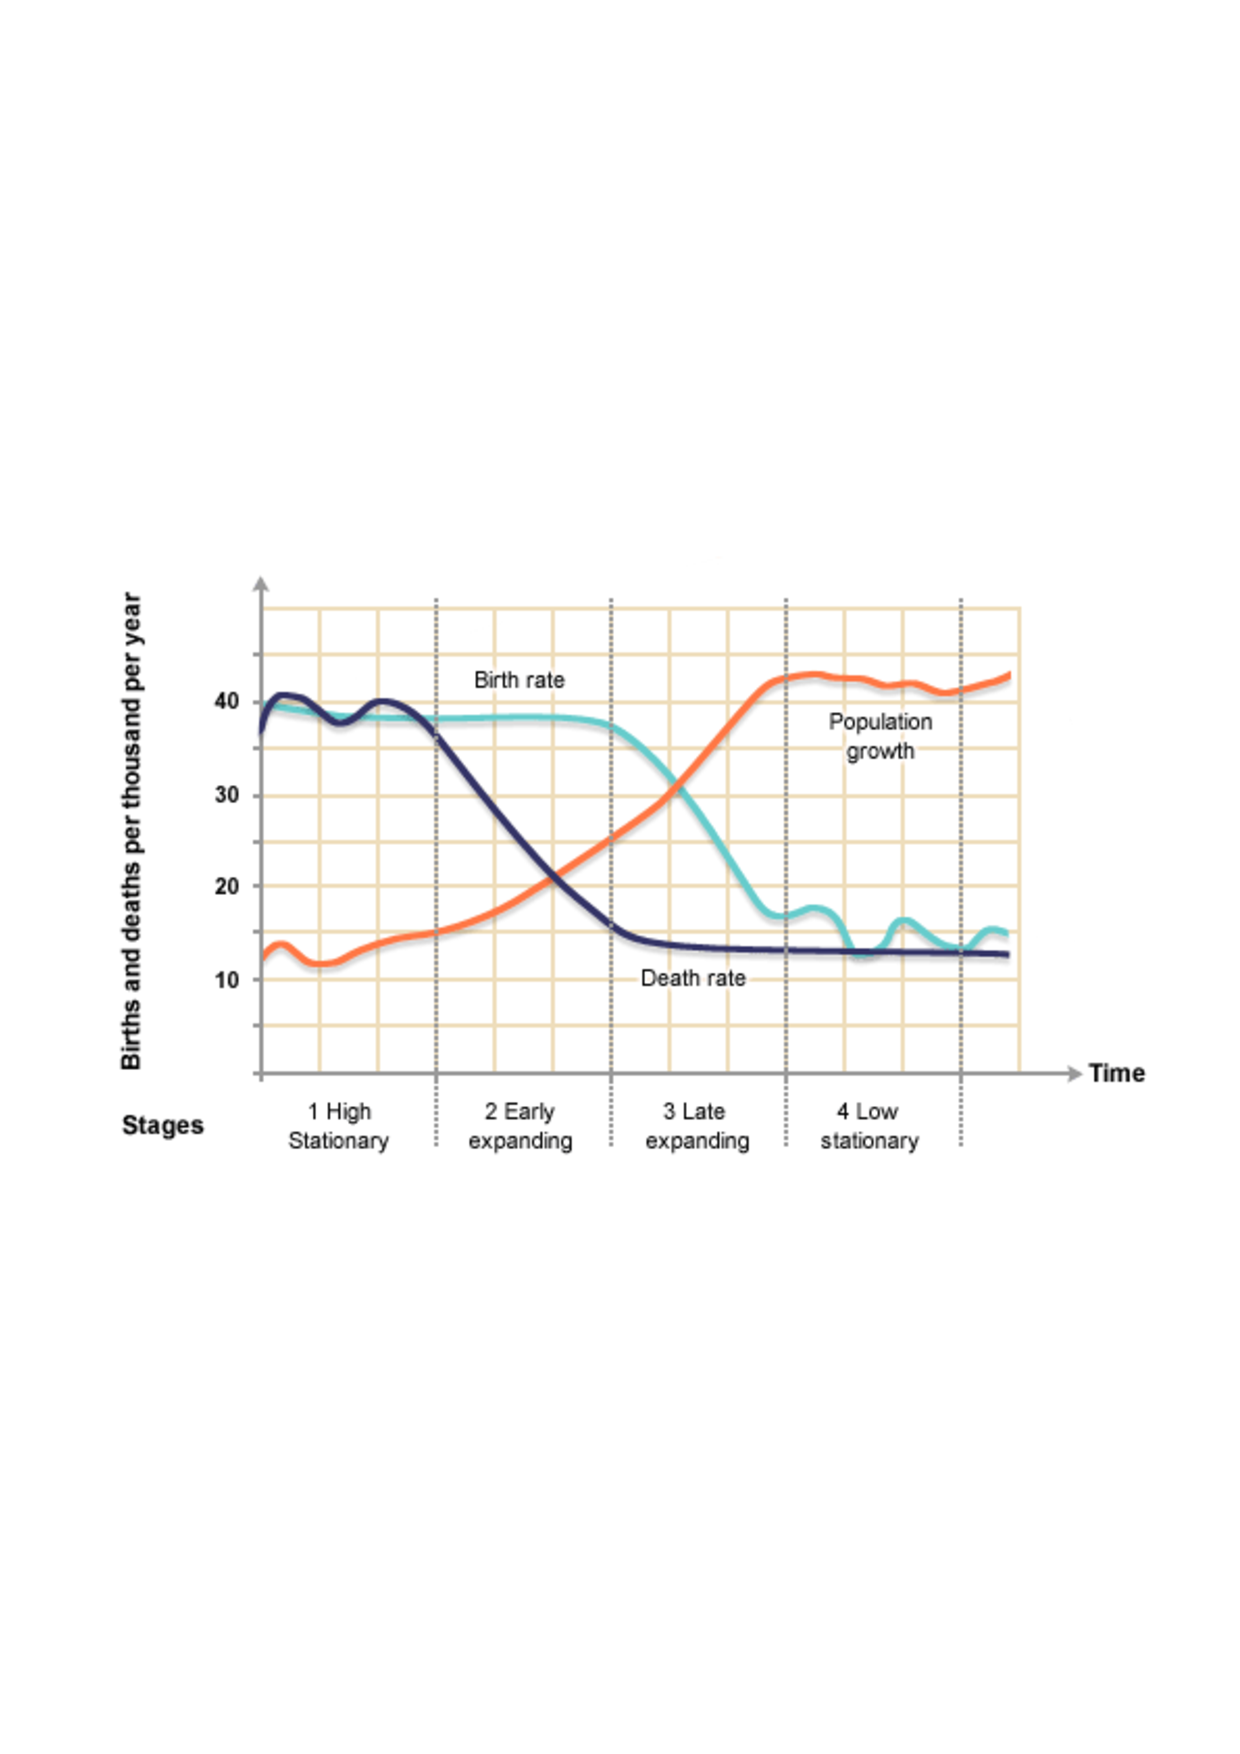
\includegraphics[width=\linewidth]{population_changes.pdf}
  \caption{The changes in the birth and death rates as well as the population growth during the transitions}
  \label{background.fig.population}
\end{figure}


\textbf{The tradition-directed type} dominates in the primitive societies, where both birth rate and death rate were high (refers to the first stage in Figure~\ref{background.fig.population}). Its members are with a low level of individualism and strong ties to primary groups, obeying rules established a long time in the past. This kind of social character has, according to Riesman, disappeared in the modern American
society, except in pockets of black, French Canadian, Southern, rural and immigrant cultures. 

Due to the drop of death rate in industrial economies (refers to the second stage in Figure~\ref{background.fig.population}), as well as industrialization, urbanization and modern technology, there was an intensive expansion of goods and people. As a result, many novel situations were presented, where a strict code could not encompass in advance like in the tradition-directed society and the control of the primary group in a tradition directed society was loosened. Therefore,~\textbf{the inner-directed type} became dominant, offering a wide choice but stable at the same time, whose members discovered the potential within themselves to live and act not according to the established norms but based on what they discovered using their own inner gyroscope that were essentially ``implanted'' by elders. Compared to the other-directed type, the inner-directed type of social character is focused on producing than consuming, whose members conform their outward behaviors, like dressing, to match societal norms, while the opinions of others have little sway on their inner lives, for example, the goal of pursuing money and rights. In other words, They would rather be esteemed than be loved.

In the mid twenties century, as the birth rate begins to follow the death rate downward (refers to the third and fourth stage in Figure~\ref{background.fig.population}), societies move toward the epoch of incipient decline of population and of service, trade and communications-driven economy. Fewer and fewer people work, hours are short, people may have material abundance and leisure besides, who are mixed more widely and thereafter becoming more sensitive to each other, since material environment is no longer a problem. Therefore, the social character was shifting from a 19th-century inner-directed type to a mid-20th-century~\textbf{other-directed type}, dominated by a concern for ``niceness'' instead of achievement, leisure instead of competition and ``consumerism'' instead of production. However, due to the lack of the cultural expectations for how to live, the other-directed people look to their peers and the media for guidance, making them very sensitive to the preferences and expectations of others using a ``radar''. Compared to inner-directed people, they would rather be loved than esteemed. In particular, modern parents and teachers are anxiety ridden as their authority over children and students has been undermined by the media, youth culture and a rapid social change that creates a situation where the ``other-directed child is often more knowing than his parents''. 


			

			
		



\chapter{Task Design and Hypothesis}
\label{chp.hypothesis}


In this chapter, we first introduce the extended Stroop task in Section~\ref{sec.hypothesis.expstrooptask} 
which is employed as a major 
instrument to explore the relationship between the ability of inhibitory control and the motherhood;
thereafter, the experiment design and three hypotheses are introduced in Section~\ref{sec.hypothesis.design} and~\ref{sec.hypothesis}.

\section{Extended Stroop Task}\label{sec.hypothesis.expstrooptask}
Recall that in the traditional Stroop task, 
as introduced in Section~\ref{subsec.measureability},
the participants are asked to name the printing color
of a word, whose literal notion (of a color)
serves as the interferences, where the Stroop effect indicates the phenomenon that a longer response time and a higher error rates are observed 
given a word with an incongruent literal notation
relative to its printing color~\citep{stroop1935studies}.
Such Stroop effect could be explained by the automatic theory as summarized in Section~\ref{subsec.measureability}, namely,
participants could automatically understand
the meaning of a word as a result of habitual reading,
whereas 
the recognition of the interfering printing color
might require a hesitation due to that the recognition 
 is not an ``automatic process''~\citep{monahan2001coloring}. 
In addition,
the traditional Stroop task has been extended 
to investigate the effects of emotional interference,
leading to the emotional Stroop task. 
Therein 
participants are asked to name the printing color of a word,
which literally denotes an emotional concept like ``hate''.
\citeauthor{algom2004rational}
argues that, however, the incongruent semantic meaning is 
missing in the emotional Stroop task, which lies at the heart of the 
original Stroop task,
making the observed effect different from a Stroop effect~\citep{algom2004rational}.


In this work,
to incorporate the emotional interference in a Stroop task,
inspired by the emotional interference tasks~\citep{otte2011interference,lee2007controlling}, 
an extended Stoop task is proposed.
According to~\citep{dimberg2000unconscious,lundqvist1995facial,wild2001emotions},
the procedure to simulate a facial expression (with a facial expression)
is also ``automatic process'',
whereas a facial expression in response to a word is not habitual.
Consequently,
corresponding to the printing color of a word and its literal notation 
from the original Stroop task respectively,
in the extended Stroop task,
we ask a participant to make a facial expression according to a word, which is 
displayed together with an interfering picture including an emotional facial expression. 
In particular, a participant is asked to simile or frown 
in response to a word, namely, 
either ``happy'' or ``angry'', 
meanwhile a photo including a happy or angry facial expression with 
the same or different emotion, 
denoted as ``positive'' and ``negative'' respectively, 
serves as interference. 
To further investigate the impact of the interaction between a mother and a baby over the inhibitory control,
the distracting facial expressions from 
both adults and babies are introduced.
For example, as displayed in Figure~\ref{fig.method.task},
a word ``happy'' as well as an angry facial expression from a baby are displayed, 
where a smile is expected from the participants 
as a correct response
according to the word ``happy''.

% this is for method chapter
% Electromyography(EMG), an experimental technique for evaluating and recording the electrical activity produced by skeletal muscles, becoming a standard tool in the study of the production of the facial expressions. Akin to \citeauthor{otte2011interference} as well as to \citeauthor{lee2007controlling}, Electromyography (EMG) is employed in the extended Stroop Task to measure the correctness and the response time (RT) of the facial expression from a subject by capturing the movements of two groups of facial muscles, namely, the zygomatic major muscle controlling smiling and the corrugator supercilii muscle controlling frowning \citep{otte2011interference,lee2007controlling}.


\section{Experimental Deign}\label{sec.hypothesis.design}
\begin{table}[!t]
\centering
% change the vertical space, 1.0 is the standard 
\ra{1.7}
\caption{Experiment conditions for the group of mother ($m1\cdots m8$,)  and non-mother ($n1\cdots n8$ ), indicating the number for the 8 different conditions in each group.}
\label{tab.hypothesis.whole.design}
% change the overall size 
\resizebox{0.7\textwidth}{!}{
% @{} remove the space at two sides
\begin{tabular}{@{}ccc|cc@{}}
\toprule
\multicolumn{3}{c|}{experiment conditions}& adults' faces &babies' faces\\
\midrule
\multirow{4}{*}{mother}&\multirow{2}{*}{positive}&``Freude''&$M_1$&$M_2$\\
&&``Ärger''&$M_3$&$M_4$\\
% \cmidrule{2-5}
&\multirow{2}{*}{negative}
&``Freude''&$M_5$&$M_6$\\
&&``Ärger''&$M_7$&$M_8$\\
\cmidrule{1-5}
\cmidrule{1-5}
\multirow{4}{*}{non-mother}&\multirow{2}{*}{positive}&``Freude''&$N_1$&$N_2$\\
&&``Ärger''&$N_3$&$N_4$\\
% \cmidrule{2-5}
&\multirow{2}{*}{negative}
&``Freude''&$N_5$&$N_6$\\
&&``Ärger''&$N_7$&$N_8$\\
\bottomrule
% \multirow{4}{c}{the group of non-mother}\\
\end{tabular}
}
\end{table}
In this work,
to examine the differences in the ability of inhibitory control between mothers and non-mothers, 
the responses from the participants to the German word \textit{Freude} (happy) or \textit{Ärger} (angry)
are recorded
when being distracted by a facial picture from 
a \textit{baby} or an \textit{adult} with a \textit{positive} or a \textit{negative} facial expression.
The responses are further examined in terms of the response time 
and the accuracy where a response is correct if it follows the displayed word and vice versa as indicated in Figure~\ref{fig.method.task}.
In particular,
the identity of a facial picture (namely, an adult or a baby),
the desired response indicated by the words (namely, ``Freude'' or ``Ärger''),
and the emotion expressed on the interfering facial picture (namely, a positive or negative emotion) are independent variables,
leading to eight different experiment conditions;
meanwhile,
the motherhood (namely, a mother or a non-mother)
is another independent variable, enabling the comparison.
Given one of the eight experiment conditions,
the response from a participant is recorded in terms of  
the response time and the accuracy, which are the dependent 
variables to quantify the ability of the inhibitory control,
constituting an \textit{experiment trial}.
According to the experiment setting,
the identification of the participant (namely, either a mother or a non-mother),
all trials are sub-clustered into sixteen subsets as summarized in 
Table~\ref{tab.hypothesis.whole.design}.
At the end of this section, 
to facilitate our descriptions,
several notations are defined in the following.


\textbf{Notation.}
Individual trials in our experiments are denoted as $t_i\in T$, 
where $T$ represents the set of all trials. 
As defined in Table~\ref{tab.hypothesis.whole.design}, 
the sixteen subsets of $T$ are $M_1\cdots M_8$ for the group of mother 
and $N_1\cdots N_8$ for the group of non-mother.
Furthermore, given a subset $T^\prime\subset T$, the average accuracy and the average response time among all $t_i \in T^\prime$ are defined as $\mathit{accuracy}(T^\prime)$ and $\mathit{rtime}(T^\prime)$ respectively. 
I further denote several subsets of $T$: they are 
$T_{mc}$, $T_{mi}$, $T_{nc}$, and $T_{ni}$, as defined in Table~\ref{tab.hypothesis.1},
which will be used in hypothesis 1;
$T_{bc}$, $T_{bi}$, $T_{ac}$, and $T_{ai}$ in Table~\ref{tab.hypothesis.2} for hypothesis 2;
and $T_{mbc}$, $T_{mbi}$, $T_{mac}$, $T_{mai}$, $T_{nbc}$, $T_{nbi}$, $T_{nac}$, and $T_{nai}$ for 
hypothesis 3. The meaning of these subsets are introduced in the corresponding tables and hypotheses.

		
\section{Hypotheses}\label{sec.hypothesis}
To investigate the relationship between the motherhood and the ability of the inhibitory control,
a research question to answer is that 
whether the motherhood makes one more prone to the interferences in terms of emotional facial expressions.
According to this research question, three hypotheses are stated, depending on whether the interfering facial expressions come from
an adult or a baby.
\begin{itemize}
\item[(a)] When comparing a mother with a non-mother, a mother is more prone to be distracted by the interferences in terms of emotional facial expressions.
\item[(b)] When distinguishing the source of the interferences, the interfering facial expressions from a baby and from an adult impact differently, disregarding of the status of motherhood.
\item[(c)] 
When further considering the interaction between a mother and an interfering facial expression from a baby, 
compared to a non-mother, a mother is more likely to be impacted by the emotional facial expressions from a baby.
\end{itemize}


Actually, to examine these three hypotheses, 
one could simply control some independent variables and compare the Stroop effects between (among) different groups,
namely, for hypothesis (a), the mother and non-mother is the controlled independent 
variable; similarly, to examine hypothesis (b), the source of the interfering facial expression,
namely, a baby or an adult, needs to be controlled; and for (c),
both mentioned independent variables should be controlled.

In addition,
recall that, as described in Section~\ref{sec.hypothesis.expstrooptask},
in the extended Stroop Task, the Stroop effects are 
in terms of the different responses when facing congruent or incongruent interference,
namely, 
a shorter response time and a higher accuracy 
in response to a congruent pair of word and facial picture, meanwhile a longer response time and a lower accuracy 
in response to a incongruent pair of word and facial picture.
Therefore, akin to~\citep{bugg2008multiple}, in this work,
the Stroop effect is quantified in terms of the differences 
of the response time and of the accuracy between congruent and incongruent trials.
Accordingly, three hypotheses in the context of the extended Stroop task are derived, using the notations
from Section~\ref{sec.hypothesis.design}.
\begin{table}[!t]
\centering
\ra{1.7}
\caption{Subsets defined for hypothesis 1. }
\resizebox{0.7\textwidth}{!}{
\label{tab.hypothesis.1}
\begin{tabular}{@{}cccc@{}}
\toprule
\multicolumn{2}{c}{experiment conditions}&subsets\\
\midrule
\multirow{2}{*}{mother}&congruent&$T_{mc}=M_1\cup M_2 \cup M_7 \cup M_8$\\
&incongruent&$T_{mi}=M_3\cup M_4 \cup M_5 \cup M_6$\\
\cmidrule{2-3}
\cmidrule{2-3}
\multirow{2}{*}{non-mother}&congruent&$T_{nc}=N_1\cup N_2 \cup N_7 \cup N_8$\\
&incongruent&$T_{ni}=N_3\cup N_4 \cup N_5 \cup N_6$\\
\bottomrule
% \multirow{4}{c}{the group of non-mother}\\
\end{tabular}
}
\end{table}
 
\noindent - \textbf{H1}:
As indicated in Table~\ref{tab.hypothesis.1}, 
compared with the group of non-mother ($T_{n.}$), 
the group of mothers ($T_{m.}$) are more prone to the interferences, resulting in a larger Stroop effect in the group of mothers than of the non-mothers, as formally summarized in Equation~\ref{eq.accuracy.h1} and~\ref{eq.rtime.h1}.

\begin{align}
\begin{split}\label{eq.accuracy.h1}
\mathit{accuracy}(T_{mc})-\mathit{accuracy}(T_{mi})&>
\mathit{accuracy}(T_{nc})-\mathit{accuracy}(T_{ni})\\
&\mathit{AND}\\
\end{split}\\
\begin{split}\label{eq.rtime.h1}
\mathit{rtime}(T_{mc})-\mathit{rtime}(T_{mi})<
\mathit{rtime}(T_{nc})-\mathit{rtime}(T_{ni})\\
\end{split}
\end{align}


\begin{table}
\centering
\ra{1.7}
\caption{Subsets defined for hypothesis 2.}
\label{tab.hypothesis.2}
\resizebox{0.7\textwidth}{!}{
\begin{tabular}{@{}cccc@{}}
\toprule
\multicolumn{2}{c}{experiment conditions}&subsets\\
\midrule
\multirow{2}{*}{babies'}&congruent&$T_{bc}=M_2\cup M_8\cup N_2\cup N_8$\\
&incongruent&$T_{bi}=M_4 \cup M_6 \cup N_4 \cup N_6$\\
\cmidrule{2-3}
\cmidrule{2-3}
\multirow{2}{*}{adults'}&incongruent&$T_{ac}=M_1 \cup M_7 \cup N_1\cup N_7 $\\
&incongruent&$T_{ai}=M_3\cup M_5 \cup N_3 \cup N_5$\\
\bottomrule
\end{tabular}
}
\end{table}


\noindent - \textbf{H2}:
As denoted in Table~\ref{tab.hypothesis.2},
compared with an interfering facial expression from an adult ($T_{a.}$),
a facial expression from a baby ($T_{b.}$) could lead to
a larger Stroop effect, as formally indicated in Equation~\ref{eq.accuracy.h2} and~\ref{eq.rtime.h2}.

\begin{align}
\begin{split}\label{eq.accuracy.h2}
\mathit{accuracy}(T_{bc})-\mathit{accuracy}(T_{bi})&<
\mathit{accuracy}(T_{ac})-\mathit{accuracy}(T_{ai})\\
&\mathit{AND}\\
\end{split}\\
\begin{split}\label{eq.rtime.h2}
\mathit{rtime}(T_{bc})-\mathit{rtime}(T_{bi})>
\mathit{rtime}(T_{ac})-\mathit{rtime}(T_{ai})\\
\end{split}
\end{align}

\begin{table}[!t]
\centering
\ra{1.7}
\caption{Subsets defined for hypothesis 3.}
\label{tab.hypothesis.3}
\resizebox{0.7\textwidth}{!}{
\begin{tabular}{@{}ccc|c@{}}
\toprule
\multicolumn{3}{c|}{experiment conditions}& subsets\\
\midrule
\multirow{4}{*}{mother}&\multirow{2}{*}{babies'}&congruent&$T_{mbc}=M_2\cup M_8$\\
&&incongruent&$T_{mbi}=M_4 \cup M_6$\\
%\cmidrule{3-4}
&\multirow{2}{*}{adults'}
&congruent&$T_{mac}=M_1 \cup M_7 $\\
&&incongruent&$T_{mai}=M_3\cup M_5$\\
\cmidrule{1-4}
\cmidrule{1-4}
\multirow{4}{*}{non-mother}&\multirow{2}{*}{babies'}&congruent&$T_{nbc}=N_2\cup N_8$\\
&&incongruent&$T_{nbi}=N_4 \cup N_6$\\
%\cmidrule{3-4}
&\multirow{2}{*}{adults'}
&congruent&$T_{nac}=N_1\cup N_7$\\
&&incongruent&$T_{nbi}=N_3 \cup N_5$\\
\bottomrule
\end{tabular}
}
\end{table}


\noindent - \textbf{H3}:
Compared with when a non-mother being interfered by a facial expression from an adult,
an interfering facial expression from a baby could lead to a larger Stroop effect in the group of mother.
More formally,
according to the notations from Table~\ref{tab.hypothesis.3},
the Stroop effects over four groups are involved,
namely, 
 $T_{ma.}$, $T_{mb.}$, $T_{nb.}$, and $T_{na.}$.
 In addition to hypothesis 2, this hypothesis is summarized in
 Equation~\ref{eq.accuracy.h3} and~\ref{eq.rtime.h3}.

\begin{align}
\begin{split}\label{eq.accuracy.h3}
\mathit{accuracy}(T_{mbc})-\mathit{accuracy}(T_{mbi})&>
\mathit{accuracy}(T_{mac})-\mathit{accuracy}(T_{mai})\\
\mathit{accuracy}(T_{nbc})-\mathit{accuracy}(T_{nbi})&<
\mathit{accuracy}(T_{nac})-\mathit{accuracy}(T_{nai})\\
&\mathit{AND}\\
\end{split}\\
\begin{split}\label{eq.rtime.h3}
\mathit{rtime}(T_{mbc})-\mathit{rtime}(T_{mbi})&<
\mathit{rtime}(T_{mac})-\mathit{rtime}(T_{mai})\\
\mathit{rtime}(T_{nbc})-\mathit{rtime}(T_{nbi})&>
\mathit{rtime}(T_{nac})-\mathit{rtime}(T_{nai})\\
\end{split}
\end{align}

% Therefore, the mean of incongruent condition and mean of congruent condition are calculated first in each group. According to the \ref{tab.hypothesis.whole.design}, in the group of mothers, the reaction time and accuracy rate in the conditions m1, m2, m7, m8 are merged and examined as congruent conditions (is marked as condition m-c), and ones in the conditions m3, m4, m5, m6 are merged and examined as incongruent conditions (is marked as condition m-ic). Similarly, in the group of non-mothers the reaction time and accuracy rate in the conditions n1, n2, n7, n8 are merged and examined as congruent conditions  (is marked as condition n-c), and ones in the conditions n3, n4, n5, n6 are merged and examined as incongruent conditions (is marked as condition n-ic).


% Two means are then abstracted in each group, in order to get the Stroop effect of each group, namely, in the group of mothers, the reaction time and accuracy rate in m-c condition is abstracted by the ones in m-ic condition (the result is marked as ms). Meanwhile, in the group of non-mothers, the reaction time and accuracy rate in n-c condition is abstracted by the ones in n-ic condition (the result is marked as ns). Finally, we get two means (mstroop) and (nstroop), The hypothesis establishes, if two Stroop effect from the group of mother and from the group of non-mothers are different from each other(mstroop-nstroop not eual zero), in the direction that the Stroop effect in the group of mother is larger than the one in the group of non-mother (mstroop>nstroop).





% Compared with an interfering facial expression from an adult,
% a facial expression from a baby could impact more, 
% leading to a larger Stroop effect when participants face facial expressions of babies than when they face ones of adults.

% Similarly, the mean of incongruent condition and mean of congruent condition are calculated first separately in the condition of adults' faces and in the condition of babies' faces. According to the {tab.hypothesis.whole.design}, in the condition of adults' faces, the reaction time and accuracy rate in the conditions m1, n1, m7, n7 are merged and examined as congruent conditions (is marked as condition a-c), and ones in the conditions m3, n3, m5, m5 are merged and examined as incongruent conditions (is marked as condition a-ic). Similarly, in the condition of babies' faces the reaction time and accuracy rate in the conditions m2, n2, m8, n8 are merged and examined as congruent conditions  (is marked as condition b-c), and ones in the conditions m4, n4, m6, n6 are merged and examined as incongruent conditions (is marked as condition b-ic).

% Two means are then abstracted in each condition, in order to get the Stroop effect of each condition, namely, in the condition of adults' faces, the reaction time and accuracy rate in a-c condition is abstracted by the ones in a-ic condition (the result is marked as astroop). Meanwhile, in the condition of babies' faces, the reaction time and accuracy rate in b-c condition is abstracted by the ones in b-ic condition (the result is marked as bstroop). Finally, we get two means (astroop) and (bstroop), The hypothesis establishes, if two Stroop effect in the the condition of adults' faces and in the condition of babies' faces are different from each other (bstroop-astroop not eual zero), in the direction that the Stroop effect in the condition of babies' faces is larger than the one in the the condition of adults' faces (bstroop > astroop).






% The mean of incongruent condition and mean of congruent condition are calculated first separately in each four conditions \ref{tab.hypothesis.whole.design}.

% \begin{itemize}
% \item[(1)] in the condition combining the group of mother and adults' faces, the reaction time and accuracy rate in the conditions m1, m7 are merged and examined as congruent conditions (is marked as condition m-a-c), and ones in the conditions m3, m5 are merged and examined as incongruent conditions (is marked as condition m-a-ic).

% \item[(2)]  In the condition combining the group of non-mother and and adults' faces, the reaction time and accuracy rate in the conditions n1, n7 are merged and examined as congruent conditions  (is marked as condition n-a-c), and ones in the conditions n3, n5 are merged and examined as incongruent conditions (is marked as condition n-a-ic).

% \item[(3)]  In the condition combining the group of mother and and babies' faces, the reaction time and accuracy rate in the conditions m2, m8 are merged and examined as congruent conditions  (is marked as condition m-b-c), and ones in the conditions m4, m6 are merged and examined as incongruent conditions (is marked as condition m-b-ic).

% \item[(4)]  In the condition combining the group of non-mother and babies' faces, the reaction time and accuracy rate in the conditions n2, n8 are merged and examined as congruent conditions  (is marked as condition n-b-c), and ones in the conditions n4, n6 are merged and examined as incongruent conditions (is marked as condition n-b-ic).

% \end{itemize}

% Two means are then abstracted in each four conditions, in order to get the Stroop effect of each condition.
% \begin{itemize}

% \item[(1)]in the condition combining the group of mother and adults' faces, the reaction time and accuracy rate in m-a-c condition is abstracted by the ones in m-a-ic condition (the result is marked as mastroop). 
% \item[(2)]in the condition combining the group of non-mother and adults' faces, the reaction time and accuracy rate in n-a-c condition is abstracted by the ones in n-a-ic condition (the result is marked as nastroop).
% \item[(3)]In the condition combining the group of mother and babies' faces, the reaction time and accuracy rate in m-b-c condition is abstracted by the ones in m-b-ic condition (the result is marked as mbstroop).
% \item[(4)]In the condition combining the group of non-mother and babies' faces, the reaction time and accuracy rate in n-b-c condition is abstracted by the ones in n-b-ic condition (the result is marked as nbstroop).
% \end{itemize}
% The hypothesis establishes, if the Stroop effect in these four conditions are different from each other, more specifically the Stroop effect in the condition combining the group of mothers and babies' faces (nbstroop) is the largest than other three conditions.

% \end{itemize}
% \begin{table}[!t]
% \centering
% \caption{Experiment settings for the group of mother ($m1\cdots m8$,)  and non-mother ($n1\cdots n8$ ), indicating the number for the 8 different settings in each group.}
% \label{tab.hypothesis.3}
% \begin{tabular}{c|c|c|c|c}
% \toprule
% \multicolumn{3}{c|}{experiment settings}& adults' faces &babies' faces\\
% \midrule
% \multirow{4}{*}{mother}&\multirow{2}{*}{positive}&``Freude''&m1&m2\\
% &&``Ärger''&m3&m4\\
% \cmidrule{2-5}
% &\multirow{2}{*}{negative}
% &``Freude''&m5&m6\\
% &&``Ärger''&m7&m8\\
% \cmidrule{1-5}
% \cmidrule{1-5}
% \multirow{4}{*}{non-mother}&\multirow{2}{*}{positive}&``Freude''&n1&n2\\
% &&``Ärger''&n3&n4\\
% \cmidrule{2-5}
% &\multirow{2}{*}{negative}
% &``Freude''&n5&n6\\
% &&``Ärger''&n7&n8\\
% \bottomrule
% % \multirow{4}{c}{the group of non-mother}\\
% \end{tabular}
% \end{table}


%The combination of the mother and while facing the infant facial expressions is expected to be interfered most compared to other three combinations: mother facing the adult faces, non-mother facing the adult faces and non-mother facing the baby faces. 
%More specifically, on congruent trails the combination of mother and infant faces is expected to have the smallest reactions time, highest accuracy while on incongruent trails this combination is expected to have the largest reactions time, lowest accuracy and lowest quality.


%It is well-known that a preverbal infant communicates with its mother with emotional facial expressions, and a mother distinctly pays special attentions to such expressions and is well prepared to react spontaneously, e.g., to comfort a crying baby. Thompson-Booth and his colleagues (2014) looked close into such phenomenon and demonstrated the difference between a mother and a non-mother in their attentions in front of an emotional face from an infant and from an adult, where an attentional bias is observed toward the infant face. What has not been fully explored is that whether such difference also affects the ability of inhibitory control, namely, the ability to make certain reactions in terms of facial expressions in front of a displayed facial expression. Put differently, we would like to investigate whether a mother is more likely to be interfered by an emotional face from an infant in comparison to an adult.

%Existing works have demonstrated that there exist interference effects when an adult is given an emotional face (Dimberg, Thunberg, & Elmehed, 2000; Lunqvist, 1995; Wild, Erb, & Bartels, 2001). In particular, an adult is interfered by a displayed face when being asked to response with a certain facial expression, where the displayed face degrades his/her ability in fulfilling the tasks in terms of the time and the correctness. Recall that an emotional face from an infant could trigger stronger attentions from a mother than from a non-mother (Thompson-Booth et al., 2014). Therefore, one may expect such difference in attentions could also be mirrored in terms of the ability of inhibitory controls, namely, a mother is more likely to be interfered by an infant face. In order to examine such effects, an extended Stroop task is designed and implemented in this work, where a subject, either a mother or a non-mother, is instructed to react with a certain facial expression in front of an interfering facial expression from an adult or an infant as background. The time and the correctness of the reaction are measured. 

%Most importantly, we intend to find the interaction effect of motherhood and art of interference stimuli over the ability of inhibitory control, namely, a larger Stroop effect in mothers than non-mothers when facing baby facial expressions compared to adult ones is expected. Put differently, we expect a difference in resisting the interference of  production similar facial expression towards infant emotional faces between mothers and non-mothers in either positive (concordant emotions displayed by the face and the word) or negative way (discordant emotions displayed), where mothers would be more interfered by infant emotional faces. In a word, the Stroop effect is expected to be larger in mothers than in non-mothers when facing baby faces.




\chapter{Method}\label{chp.method}

Three sections are included in this chapter. The experimental setup, the procedure of the experiment 
and the data processing procedures are introduced in details 
in Section~\ref{sec.method.setup},~\ref{sec.method.details} and~\ref{sec.method.postprocessing} respectively. 

\section{Experiment Setup}\label{sec.method.setup}
In this section, the enrollment of the participants, 
the stimuli and apparatus employed,
and the collection of the EMG data are introduced. 
The study described in this section is part of the parenthood study project supported by Deutsche Forschungsgesellschaft.
The experiment described in this section was conducted
in Psychology Institute of the Humboldt University in Campus Adlershof in Berlin. 

\textbf{Enrollment of the participants.}
In total, there were 62 female volunteers involved in our experiments by the time of writing, including 24 participants who were not raising a baby and constitute of the non-mother group, and 38 mothers who were breastfeeding a baby between two and six months and compose the mother group. Due to the problems of collected data, data from 17 non-mothers (aged 18-32, M = 24) was actually used. In order to compare the mothers and non-mothers, data from 20 mothers (aged 26-39, M = 31) was actually used.
All the participants received 40€ after the experiments for compensation.
To make sure the sanity of the collected data, telephone interviews 
were employed to screen the candidates using following criteria: A qualified participant should
\begin{itemize}
\item[-] be a female European descent for the sake of the facial expression recognition;
\item[-] be between 18 and 45 years old;
\item[-] be fluent in German, namely, on par with a native German speaker;
\item[-] not have taken medications which could influence the level of hormone;
\item[-] not have psychological disorder which could affect the perception or the production of facial expressions; 
\item[-] have normal or corrected-to-normal visual acuity.
\end{itemize}
Accordingly, all candidates were interviewed beforehand through a telephone call.
	
\textbf{The stimuli and the apparatus.}
Recall that,  
as introduced in Section~\ref{sec.hypothesis.expstrooptask},
the facial expressions from babies and from adults were employed as stimuli
in the extended Stroop task.
In particular, 
pictures include 
either positive (namely, smile) or negative (namely, cry or angry) facial expressions from 20 babies (ten girls and ten boys)\footnote{The pictures were collected from web and were rated to be highly related to the expressed emotions},
and from 20 adults (ten females and ten males)\footnote{The pictures come 
from Radboud Faces Database~\cite{langner2010presentation}.} were used.
All the pictures were normalized into a unified format to remove unrelated factors,
in terms of 
size (7cm $\times$ 9.33cm),
brightness, contrast grade (visual angle: 4.01\textdegree $\times$5.35\textdegree),
spatial frequency, and other properties. 
As for the text signals, 
German words Freude (happy) and Ärger (angry) were displayed in black color, 
superimposing on top of the facial pictures, indicating the same or the opposite facial expressions relative to the pictures. Four example pictures are displayed in Figure~\ref{fig.method.setup.example}, 
Both the facial pictures and the words were displayed in full screen on 19-inch monitors (35 cm $\times$ 25 cm), which was placed 70 cm away from the participants. 


\textbf{Record the responses from a participant.}
Different experiment conditions are summarized in Section~\ref{sec.hypothesis.design},
for which all trails were presented in random order, 
and at least 60 trials were collected for each experiment condition, 
ending up with 480 recorded trials in total.
The EMG signals from the participants
when making responses were captured. In addition,
videos of their facial expressions 
were also recorded to cross-examine the results derived from the EMG signals.
Based on the recorded EMG signals,
the response time was derived which will be introduced in Section~\ref{sec.method.postprocessing}. Besides, the electroencephalography (EEG) was also used to record the brain activity of the participants during the task, whose data was not analyzed in this work.

% and the accuracy of the response (e.g., a response is correct if it reflects the displayed word and verse visa.).

% In particular, the response from a participant
% is recored via electromyography (EMG)
% RT was measured as EMG onset latency of trials, 

%  During the experiment, the facial expressions of the participants were also recorded by the videos, which were used for double checking the quality of the data.
% RT was measured as EMG onset latency of trials, in which participants made the right facial expressions, and errors included no reactions, reactions using the incorrect muscle, or reactions were a response on both muscles in some of the trials according to the videos as well as EMG recording. The table 4.1 demonstrates the design of the experiment, showing all combinations of different factors.

\textbf{Locate and affix the electrodes for EMG recording.}
In the end, some details for recording the EMG signals are described. Recall that, as mentioned in Section~\ref{subsec.background.emg}, two electrodes were used for recording the signals from one target muscle, namely, two for the corrugator and two for the zygomaticus in our study, monitoring the muscle activity when particular facial expressions were made. Thereby, in total, four sintered silver-silver chlorid (Ag-AgCl) electrodes were in use.
Besides, 
a ground electrode is required in the EMG recording which was placed at the mid-line approximately 3-4 cm superior to the upper borders of the inner brows, akin to the configuration described in~\citep{fridlund1986guidelines}.

To attach the electrodes, 
the target skins were first 
cleaned with alcohol (Isopropylalcohol 70\%); thereafter the Electrolyte-Gel was peeled for 30 seconds to further reduce the resistance on the skin surface;
in the meantime, the head-shaped electrodes were filled with ``Abrasive Electrolyte-Gel'' without bubbles before attaching to skins using double-stick adhesive collars.  
To locate target muscles, 
we followed the descriptions from~\citep{fridlund1986guidelines}, namely,
for the corrugator, 
the participant was asked to frown and  
one electrode was affixed directly on the inner commossure of the eye fissure and another was positioned 1 cm lateral to, but slightly superior to, the first on the border of the eyebrow;
as for the zygomaticus, 
one electrode was attached on 
the midway along an imaginary line joining the corner of the mouth and the particular point on the right side, and another was placed 1 cm inferior and medial to the first (i.e. towards the mouth) along the same imaginary line (The positions of two electrodes and the ground electrode are illustrated in Figure~\ref{fig.background.emg}). The raw signal was digitized with the BrainVision recording software~\footnote{Brain Products GmbH, Munich, Germany}.
%The EMG signal was measured, rectified, and integrated using a Coulbourn V76-23a Hi amplifier. Low- and high-pass filters were set at $10 kHz$ and $8 Hz$, respectively. 
		

\begin{figure}[!t]
  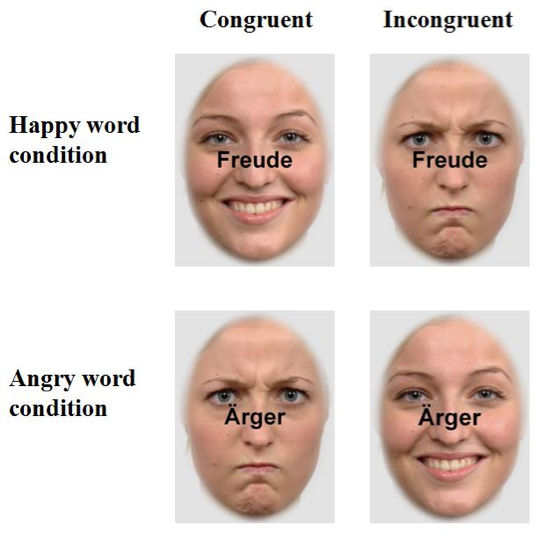
\includegraphics[width=0.9\linewidth]{pictures/Stimulus.png}
  \caption{An Example of face-word compound stimuli. The superimposing word indicates the requested facial expression from the participants, whereas the irrelevant facial pictures are displayed in the background. Up to the congruency between the word and the facial picture, there exist in total four combinations.
}
  \label{fig.method.setup.example}
\end{figure}


\section{Procedure}\label{sec.method.details}
In this section, 
the experiment details are 
described in sequence.


\noindent - \textbf{Before the task}, 
a participant was informed about the details via an information sheet, and was 
asked to complete a consent form and a demographic questionnaire (including a handedness questionnaire) whose templates are included in Appendix A and B respectively. Thereafter, the participant was seated on a comfortable chair in a soundproof and dimly-lit room. After the preparations of the electrodes, lasting about an hour, two other tasks were conducted for about a half hour before the Stroop task.

\noindent - \textbf{During the Stroop task,}
as explained in Section~\ref{sec.hypothesis.expstrooptask},
a participant was asked to response as soon as possible with a facial expression according to
the displayed word. They were also instructed to avoid making a hybrid
facial expression, namely, smiling and frowning at the same time,
which could result in invalid data.
Specifically, in each trial,
a fixation is first displayed for 500 ms,
thereafter, either ``Freude'' or ``Ärger'' is displayed in the center of 
a facial picture from a baby or from an adult with a positive or negative 
emotion for 2000 ms, during which the participant should response with 
a facial expression according to the word, until the sign ``stop'' is displayed when the participant should 
relax his(her) facial muscles returning to a neutral facial expression (an example is
displayed in Figure~\ref{fig.method.sequence});
% At the beginning of each trial, a fixation cross appeared on the screen for 500 ms. After the fixation, the face-word compound stimuli, namely a word ``happy'' or ``angry'' with either a `happy' or an `angry' facial expression of either baby or adult faces in the background, appeared in the center of the screen, which were visible for 2000 ms, during which participants could response to the words (i.e., Freude, Ärger) with facial expressions. When the `stop' signal appeared (900-1000 ms randomized), participants were instructed to relax their facial muscles and display neutral facial expression (see the Figure 4.3). 

\noindent - \textbf{Training and monitoring.}
Prior to the actual experiments, 
participants could familiarize themselves within the 
first eight trials, with which the EMG signals and the 
response patterns were also double-checked. 
During the tasks,
the procedure was monitored by our researchers from outside. Since the questionnaires for mothers are in terms of the baby, the mothers were asked to bring their baby with them to the lab. During the experiment, the babies were being taken cared and were outside the experimental room, avoiding 
their influences to the mothers from their own babies.
After every eighty trials, 
biscuits and water were offered to the participants for a break.


\noindent - \textbf{After the task,}
the second part of the questionnaire including two questions about the concentration and concerns during the Stroop task was filled (Appendix C for non-mothers and Appendix D for mothers). Each statement has four options: not at all, a little, quite and very. This self-evaluation of the concentration and concerns was used to cross examine the sanity of the data. The Stroop task (ca. 60‐min duration) was the third task, after which there was another task lasting for an hour. The whole experiment including the preparation and four tasks lasting for about four hours, including the pauses in between. At the end of the experiment, the participants were given 40€ as compensation.

% Abbildung 1

\begin{figure}[!t]
\centering
  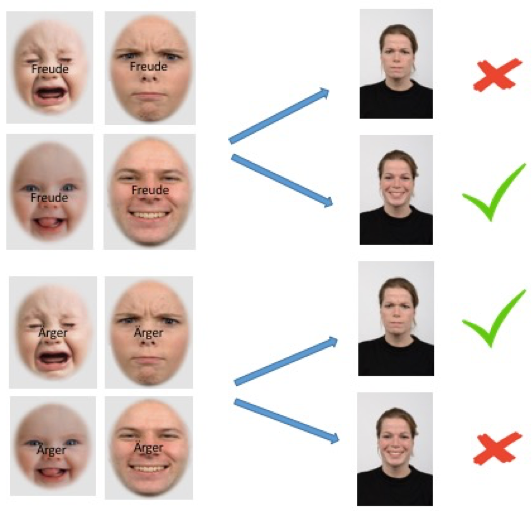
\includegraphics[width=0.9\linewidth]{pictures/Extended_Stroop_Task.png}
  \caption{Examples of the correct and wrong responses from a participant under different experiment conditions.
}
  \label{fig.method.task}
\end{figure}


\begin{figure}[!t]
  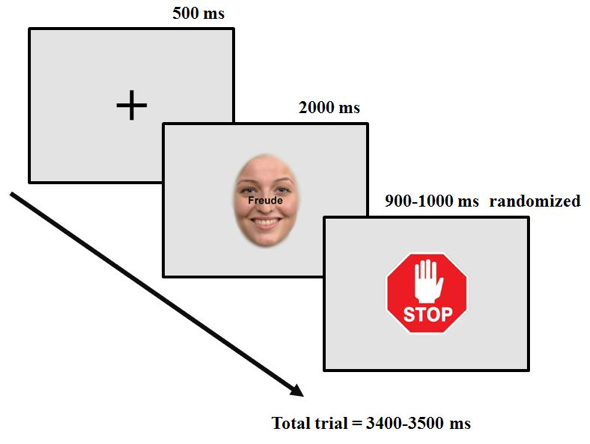
\includegraphics[width=0.9\linewidth]{pictures/One_Trial.png}
  \caption{Example of the sequences of scenes in one trial.
}
  \label{fig.method.sequence}
\end{figure}

\section{Data Processing}\label{sec.method.postprocessing}
\textbf{Post-processing of EMG data.}
Brain Vision Analyzer Software\footnote{Version 2.0, Brain Products Inc., Gilching, Germany} was used in the analyses of the EMG activity. 
The EMG signals were first filtered with a 50 Hz notch filter of the Zero Phase Shift Butterworth Filters (IIR Filters) to remove a narrow frequency band. 
The filtered EMG signals were further segmented. In particular, using the appearance of the 
stimulus, namely, the first occurrence of the word and the facial picture in a trial, as the~\textit{reference point}, and the interval between 200ms before and 2000ms after this reference was regarded as the span of the signal sequence in a trial. 
In measuring the activation of the muscles, 
in individual trials,
the strength of the signals on the first 200ms (namely, before the reference point) were regarded as baseline, corresponding to when no muscle activity presents.
According to the previous study~\citep{recio2014should}, a threshold relative to the baseline was determined by using the average strength plus 25 times of standard deviation,
which applied for all the participants. This threshold was used to determine the onset of activation of the target muscles, namely, the point in time where the amplitude in a given muscle reached 25\% of the individual maximal value of that muscle in the average was determined as the EMG onset for each trial~\citep{recio2014should}.


\textbf{Extraction of correctness.}
After processing the EMG, 
the triggered muscles, together with its activating time, were extracted, and associated
with the experiment conditions (namely, a particular type of stimulus).
Accordingly, 
the correctness of a recorded response 
could be determined by examining the EMG signals 
for the particular muscles and the displayed word, e.g., the response is correct if a EMG signal for the muscle zygomaticus exceeds the threshold while the one for the muscle corrugator doesn't, when the  ``Freude'' is displayed. 
Note that, 
if EMG signals for both muscles are below or above the threshold at the same time, the response is judged as incorrect.  

%was measured in some of the trials. There were two conditions when both muscles activated in the same time. In one condition, the wrong muscle activated first and then the right one. While in the other condition, the right muscle activated first and then the wrong one, indicating the uncertainty of the participants. The former was marked as wrong actions, while the latter was also marked as wrong actions for most of the participants in order to get the pure data. However, for nine participants (Seven mothers and two non-mothers) with more than 20 such trials, each trial was evaluated depending on the video recorded during the experiment.


\textbf{Extraction of response time.}
The latency of the first signal exceeding the 
threshold relative to the reference point was regarded as the response time.
According to the pilot experiments, 
a response time is valid only when it is between 70ms and 1000ms,
so that the erroneous records are filtered out. 
Intuitively, it is meaningful to analyze the 
response time only when a correct response presents, 
given that an incorrect response may due to a different mixture of conditions than a correct one.
Therefore, we did not want to mix up different kinds of processes and considered only the reaction time from correct trials.


\textbf{Statistic analysis.}
Given the extracted accuracy rate and the response time,  
statistical instruments were employed to examine the hypothesizes described in Section~\ref{sec.hypothesis}.
We first provide descriptives of the collected data by calculating 
several descriptive statistics. To start with, we confirmed that the collected accuracy and response time from different participants all centralize 
around the average, locating in the span between 
negative to positive
three standard deviation around the mean value. 
In addition, the average accuracies for individual participants over different experiment conditions (namely, for each participant, eight average accuracies were examined) are all above 0.5. Both observations indicate that
the participants understand the instructions well and adhere to them during the tasks.

In the following, the statistical tests are described, which are implemented with SPSS\footnote{IBM Corp. Released 2016. IBM SPSS Statistics for Windows, Version 24.0. Armonk, NY: IBM Corp.}. 
A significance level at 0.05 is reported in all tests.
% After each test, the descriptive statistics are analyzed, so that we could determine the direction of the differences.

%As a precondition of applying the mixed ANOVA, the between- and within-subjects are proved to be both independent and nominally scaled. The Greenhouse–Geisser adjustment is used to correct for violations of sphericity. There is homogeneity of the error variances, as assessed by Levene’s test (p > .05) and homogeneity of covariances, as assessed by Box’s test (p > .05). Alpha level of 0.05 is used to determine statistical significance. 
%As the premise of the experiment, we intend to examine that the Stroop effect exists in our study. Therefore, we first merge the $m1$, $m2$, $m7$, $m8$ as well as $n1$, $n2$, $n7$, $n8$ as the congruent conditions, and the $m3$, $m4$, $m5$, $m6$ as well as $n3$, $n4$, $n5$, $n6$ as incongruent conditions regardless of mothers and non-mothers. A paired t-test is conducted in order to investigate whether the Stroop effect is found.

\noindent - \textbf{Test for Stroop effect}.
Before examining the hypothesizes,
we first demonstrated the extended Stroop effect, namely,
among all trials,
a shorter (longer) response time and a higher (lower) accuracy rate
when the word and the facial expression are congruent(incongruent),
examining the designed extended Stroop task and the collected data.
A paired sample t-test was employed between 
$M_1\cup M_2\cup M_7\cup M_8\cup N_1\cup N_2\cup N_7\cup N_8$ and
$M_3\cup M_4\cup M_5\cup M_6\cup N_3\cup N_4\cup N_5\cup N_6$ from Table~\ref{sec.hypothesis.design},
where the congruency was considered as independent variable. 

\noindent - \textbf{Test for hypothesis 1}.
Recall that, in this hypothesis, we intend to investigate whether the Stroop effect is larger in the group of mother than of non-mother. Accordingly, an unpaired t-test was used, 
where the Stroop effect becomes the dependent variable and 
the status of motherhood (namely, being a mother or a non-mother) is an independent variable. 
Given the different sample sizes of the two groups (17 non-mothers and 20 mothers), 
the Welch's-test instead of the Student's t-test was employed. 
When further considering the types of the interferences, namely,
a positive (a smiling face) or a negative (a crying/frowning face), a Welch's test was also used to compare the difference of the Stroop effect between mother and non-mother when being provided a positive or a negative interference.

\noindent - \textbf{Test for hypothesis 2}.
Herein we intend to investigate whether the Stroop effect is larger when participants face the facial expressions from babies compared with when the adults' are displayed. A paired t-test was employed 
where the Stroop effect is the dependent variable, meanwhile the source of the interfering facial expression, namely a baby or an adult, is an independent variable. When combining the positive and negative interferences, we also investigated whether a negative or a positive interference from a baby leads to a larger Stroop effect compared to one from an adult using paired t-tests.


\noindent - \textbf{Test for hypothesis 3}.
In this hypothesis, a larger Stroop effect is expected 
when the mothers face the facial expressions from a baby. A paired t-test was used in the group of mother to compare the difference between the situations when the mothers are interfered by the babies and
by the adults, which was also conducted in the group of non-mother. We further consider the experiment conditions
when positive and negative interferences
were employed using paired t-test in the group of mother, namely, in front of a positive interference (smile), whether there is difference in the Stroop effect of a mother when the facial expression comes from a baby or an adult, meanwhile, whether the difference also exists, when being interfered by a negative one (frown or cry).



\chapter{Results}\label{chp.results}
In this chapter, the results are summarized and analyzed. 
In Section~\ref{sec.results.overview},
some descriptive statistics are provided, and 
the Stroop effects on different experiment groups from 
Table~\ref{tab.hypothesis.whole.design} are examined;
in addition,
the hypothesizes described in Section~\ref{sec.hypothesis} are tested per items in Section~\ref{sec.results.hypothesis}.



\section{Overview}\label{sec.results.overview}
\begin{table}[!b]
\centering
\ra{1.7}
\caption{Overall statistics for accuracy rate and response time. In addition,
the two-tailed p-value from a paired t-test is also reported.}\label{tab.results.overview}
\resizebox{0.7\textwidth}{!}{
\begin{tabular}{@{}cccc@{}}
\toprule
		& mean (congruent) & mean (incongruent) & p-value \\
   \midrule
accuracy&$0.89$&$0.83$&$p < 0.001$\\
response time&$503.2$~ms&$537.8$~ms&$p < 0.001$\\
\bottomrule
\end{tabular}
}
\end{table}



\begin{table}[!t]
\centering
\ra{1.7}
\caption{The accuracy rate with (SD) for the production of facial expressions in the different conditions.}
\label{tab.results.accuracyrate}
\resizebox{0.7\textwidth}{!}{
\begin{tabular}{@{}ccc|cc@{}}
\toprule
\multicolumn{3}{c|}{experiment conditions}& adults' faces &babies' faces\\
\midrule
\multirow{4}{*}{mother}&\multirow{2}{*}{positive}&``Freude''&$0.91(0.06)$&$0.91(0.08)$\\
&&``Ärger''&$0.87(0.08)$&$0.82(0.12)$\\
%\cmidrule{2-5}
&\multirow{2}{*}{negative}
&``Freude''&$0.82(0.10)$&$0.86(0.10)$\\
&&``Ärger''&$0.89(0.11)$&$0.87(0.11)$\\
\cmidrule{1-5}
\cmidrule{1-5}
\multirow{4}{*}{non-mother}&\multirow{2}{*}{positive}&``Freude''&$0.90(0.05)$&$0.89(0.07)$\\
&&``Ärger''&$0.82(0.12)$&$0.83(0.13)$\\
%\cmidrule{2-5}
&\multirow{2}{*}{negative}
&``Freude''&$0.80(0.10)$&$0.83(0.08)$\\
&&``Ärger''&$0.88(0.10)$&$0.87(0.10)$\\
\bottomrule
% \multirow{4}{c}{the group of non-mother}\\
\end{tabular}
}
\end{table}

\begin{table}[!t]
\centering
\ra{1.7}
\caption{The response times with (SD) for the production of facial expressions in the different conditions.}
\label{tab.results.responsetime}
\resizebox{0.7\textwidth}{!}{
\begin{tabular}{@{}ccc|cc@{}}
\toprule
\multicolumn{3}{c|}{experiment conditions}& adults' faces &babies' faces\\
\midrule
\multirow{4}{*}{mother}&\multirow{2}{*}{positive}&``Freude''&$499.3(81.1)$&$487.4(83.1)$\\
&&``Ärger''&$547.2(83.8)$&$554.7(85.5)$\\
%\cmidrule{2-5}
&\multirow{2}{*}{negative}
&``Freude''&$533.1(80.5)$&$537.3(95.3)$\\
&&``Ärger''&$492.3(80.7)$&$506.6(80.3)$\\
\cmidrule{1-5}
\cmidrule{1-5}
\multirow{4}{*}{non-mother}&\multirow{2}{*}{positive}&``Freude''&$509.8(74.5)$&$522.8(77.4)$\\
&&``Ärger''&$548.6(86.8)$&$554.5(100.8)$\\
%\cmidrule{2-5}
&\multirow{2}{*}{negative}
&``Freude''&$565.2(81.6)$&$553.9(82.8)$\\
&&``Ärger''&$496.7(79.7)$&$515.6(84.5)$\\
\bottomrule
% \multirow{4}{c}{the group of non-mother}\\
\end{tabular}
}
\end{table}


In this section, the average accuracy rate and response time among all participants
under congruent and incongruent experiment conditions
are summarized in Table~\ref{tab.results.overview}.
It can be seen that, under both conditions,
the participants achieve a reasonable accuracy, namely, beyond $0.8$, within around half seconds on average.
In addition, 
recall that the extended Stroop Task described in Section~\ref{sec.hypothesis.expstrooptask} 
actually stems from the automaticity theory~\citep{monahan2001coloring}.
Henceforth,
the Stroop effects are further examined among all participants,
namely, the different responses when the congruent and incongruent experiment conditions
are compared.
In particular,
paired t-tests 
are employed to compare both accuracy and response time separately between the two experiment conditions.
It turns out that, as expected, for both there exist significant differences
as summarized in Table~\ref{tab.results.overview},
demonstrating that the participants in general require longer time,
meanwhile tend to achieve lower accuracy under an incongruent experiment setting.
Furthermore, the accuracy and response time are displayed in 
Table~\ref{tab.results.accuracyrate} and~\ref{tab.results.responsetime} respectively for all different experiment
conditions in Table~\ref{tab.hypothesis.whole.design},
providing a detailed overviews of the results.
It can be seen that
the highest accuracy (0.91) and the shortest response time (487ms)
are recorded under the setting when mothers respond to 
``Freude'' under
a congruent interference from a smiling baby face (positive);
meanwhile, 
upon an incongruent interference (negative)
from an adult face,
a non-mother 
is more prone to make mistakes (0.80) and consume more time to react (565ms) in response to ``Freude''.
Therefore, in terms of the extreme values, 
the results for the accuracy and the response time are 
consistent. It may also imply that 
a non-mother tends to be interfered more by an adult,
whereas a mother is more sensible to the interference from babies' face.


\section{Examine Hypothesizes}\label{sec.results.hypothesis}
%interaction among motherhood, target expressions and interference expressions
\noindent - \textbf{H1}:
\textbf{Compared with non-mother, 
mothers are more prone to the interferences, resulting in a larger Stroop effect (refer to Equation~\ref{eq.accuracy.h1} and~\ref{eq.rtime.h1}).}

As mentioned in Section~\ref{sec.method.postprocessing},
a Welch's test is employed. 
The difference between the Stroop Effects from the mothers and from the non-mothers is significant for neither accuracy nor response time.  
In particular, for the mothers,
the differences of the accuracy and the response time 
between congruent and incongruent conditions 
are $0.056$ and $46.650ms$ respectively;
whereas for non-mother the differences are
$0.066$ and $44.329ms$.
The two-tail p-value for accuracy is
$0.672$ ($T(145)=-0.424$), and for response time is
$0.817$ ($T(131)=0.232$).
When further considering the types of the interferences, namely,
a positive (a smiling face) or a negative (a crying/frowning face),
the difference of the Stroop effect on response time between mother and non-mother when being provided a positive interference is not negligible, where the Stroop effect for the response time for mothers is 
$57.6ms$ and is $35.2$ for non-mother, leading to two tailed $p = 0.122$ ($T(64)= 1.569$). The similar difference is not found, when a negative interference is provided.

Therefore, the hypothesis is not supported by the data in general,
suggesting that 
the status of being a mother or a non-mother
seems not to impact the ability of the inhibitory control.
However, we do find that a mother is more prone to a positive interference compared with a non-mother.


\noindent - \textbf{H2}:
\textbf{
Compared with an interfering facial expression from an adult,
a facial expression from a baby could result in
a larger Stroop effect, as indicated in Equation~\ref{eq.accuracy.h2} and~\ref{eq.rtime.h2}.}

A paired t-test is employed.
For both accuracy and response time,
no significance is observed when comparing the Stroop effects.
In particular,
when being interfered with the facial expressions from an adult,
the Stroop effect for the accuracy and the response time  
are $0.07$ and $48.6ms$ respectively; as for the facial expressions from a baby,
the numbers are $0.05$ and $42.6ms$.
The two-tailed p-value for the accuracy is 
$p=0.194$ ($t(73)= 1.310$), and 
is $p = 0.215$ ($t(73)= 1.252$) for the response time.
When combining the positive and negative interferences, however,
the negative interference from an adult leads to larger Stroop effects
in terms of both accuracy ($0.08$ vs $0.03$) and 
response time ($53.5ms$ vs $34.2ms$),
leading to $p=0.002$ ($T(36)= 3.283$) and $0.001$ 
($T(36)=3.575$) respectively.

Henceforth, there exist no evidence to support that the interferences from an adult or a baby could lead to significantly
different Stroop effects. However, the negative facial expression from an adult (frown) does impact more than the negative expression from a baby (frown or cry).


\noindent - \textbf{H3}:
\textbf{
Compared with when a non-mother being interfered by the facial expression from an adult,
an interfering facial expression from a baby could lead to a larger Stroop effect in the group of mother, as summarized in Equation~\ref{eq.accuracy.h3} and~\ref{eq.rtime.h3}.}

In this hypothesis, the status of mother and the interference from
a baby or from an adult are co-considered, 
exploring the Stroop effects when a mother is interfered by the 
facial expression from a baby. In favor of the description,
three observations are listed in the following.

\begin{itemize}
\item[(1)] 
No significant difference between the situations
when the mothers are interfered by the babies and
by the adults.
In particular,
the two-tailed p-value for the Stroop effect
on the accuracy ($0.06$ vs $0.06$) is 
$p=0.884$ ($T(39)=-0.147$) and on the response time
($49.0ms$ vs $44.3ms$)
is $p=0.512$ ($T(39)=0.662$).

\item[(2)] 
Significant differences of the Stroop effects
for both accuracy and response time when 
a non-mother is interfered by the facial expressions from 
a baby or from an adult. 
In particular, 
when being interfered by the facial expression from a baby,
the Stroop effect of the accuracy from non-mothers is $0.05$ and 
the of response time is $35.0ms$;
whereas in front of the facial expression from an adult,
the Stroop effect of the accuracy becomes $0.08$ and 
the of response time becomes $53.6ms$,
where the differences in between are significant 
with $p=0.056$ ($T(33)=-1.981$) and 
$p=0.003$ ($T(33)=-3.233$) for the Stroop effect of the accuracy and the response time respectively.

\item[(3)]
We further consider the experiment conditions
when positive and negative interferences
are employed, whose results are summarized 
in Figure~\ref{fig.results.add}.
It turns out that,
in front of a positive interference (smile),
the mother achieves $0.10$ and $0.05$ respectively in terms of the Stroop effects of the accuracy 
when the facial expression comes from a baby and an adult,
leading to $p=0.041$ ($T(19)=2.190$);
meanwhile, when being interfered by a negative interference 
(frown or cry),
the Stroop effects of the accuracy are $0.01$ and $0.07$ in front of 
the expression from a baby or an adult,
where $p=0.010$ ($T(19)= -2.870$). However, the similar Stroop effects of the response time in the group of mother are not found. As for the non-mother, there is no difference whether the positive or negative interferences come from a baby or an adult in terms of the accuracy as well as the response time~\ref{fig.results.add}.


% \item[(3)]
% As for the comparisons between the mothers and 
% the non-mothers when being interfered by the babies or the adults,
% there exist no significant difference
% though absolute differences can be observed in Figure~\ref{fig.results.h3}.

\end{itemize}

In short, according to finding (1), 
the non-mothers are more prone to be interfered by the facial expressions
from the adults, whereas the mothers seem to behave similarly
in front of different kinds of interferences as indicated 
in finding (2). However, 
according to finding (3),
we can conclude that the mothers' ability of 
inhibitory control actually depends on the
property of the interference, namely,
in front of a positive (smile) interference,
the mothers are influenced more by the facial expressions from babies;
whereas the ones from adults influence more when a negative 
interference (frown or cry) is given.
On one hand, 
the behavior from the non-mothers may simply
comes from the daily life, namely, people is tuned
to be sensible in noticing and reacting to the facial expressions
from other adults,
which is arguably very important to behave properly
in daily works,
ending up with a lower ability of inhibitory control
in front of the facial expressions from other adults; 
Meanwhile, as for the mothers,
their behaviors are heavily tuned during their daily catering of 
the baby, making their ability of inhibitory control
differs from the one of the non-mothers.


% The results suggest the emotions of the facial expressions has an influence over the interaction of the status of the motherhood and the source of the facial expressions. More specifically, there exist an interactions effect among the status of the motherhood (mother vs. non-mother), the emotions of the facial expressions (positive vs. negative) and the source of the facial expressions (babies' and adults' faces).

% There are two reasons, which could explain the negligible difference in the Stroop effect between when babies' faces are displayed and when adults' faces are displayed in the group of mothers. One is the larger interference effect of the adults' faces towards mothers than non-mothers, which is found according to the results of a Welch's test, used to compare the differences in the Stroop effect between group of mothers and group of non-mothers when facing the adults' faces. 


% The adults' faces are found to have a larger interference effect on the group of non-mothers ($M=0.081$, $SD=0.118$) than the group of mothers ($M=0.058$, $SD=0.138$) according to the accuracy; $t(71.992)= 0.773$, $p = 0.442$. a larger interference effect of the adults' faces on the group of non-mothers ($M=53.649$, $SD=65.373$) than the group of mothers ($M=44.307$, $SD=57.132$) is also found according to the response time; $t(66.161)= 0.6492$, $p = 0.519$. 


% Although neither of them is significant. The other reason is that, the babies' faces may have a larger interference effect on the group of mothers than the group of non-mothers. 

% According to the results of a Welch's test, used to compare the differences in the Stroop effect between group of mothers and group of non-mothers when facing the babies' faces. The babies' faces are found to have a larger interference effect on the group of non-mothers ($M=0.051$, $SD=0.112$) than the group of mothers ($M=0.0552$, $SD=0.159$) according to the accuracy; $t(69.852)= 0.148$, $p = 0.883$. a larger interference effect on the group of non-mothers ($M=35.009$, $SD=64.908$) than the group of mothers ($M=48.993$, $SD=52.706$) is also found according to the response time; $t(63.483)= 1.006$, $p = 0.318$ as illustrated in Figure~\ref{fig.results.h3}. However, neither of them is significant.

% To conclude, the results suggest that there may exist an interaction between the status of the motherhood and the source of the facial expressions of the interference, which is not strictly found according to our results.

% \begin{figure}[!t]
%   \centering
%   \begin{subfigure}[b]{0.4\linewidth}
%     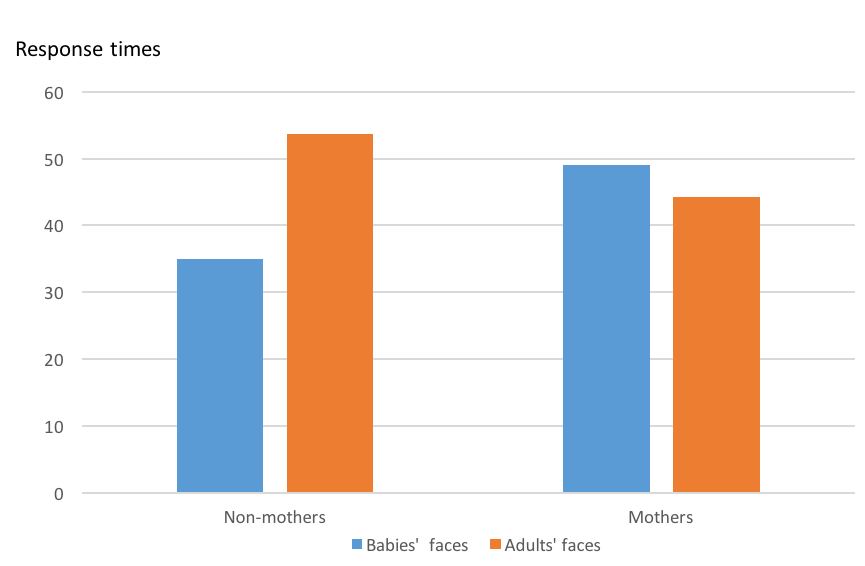
\includegraphics[width=\linewidth]{pictures/RT_identity_motherhood.png}
%     \centering
%     \caption{Stroop effect of response times}
%   \end{subfigure}
%   \begin{subfigure}[b]{0.4\linewidth}
%     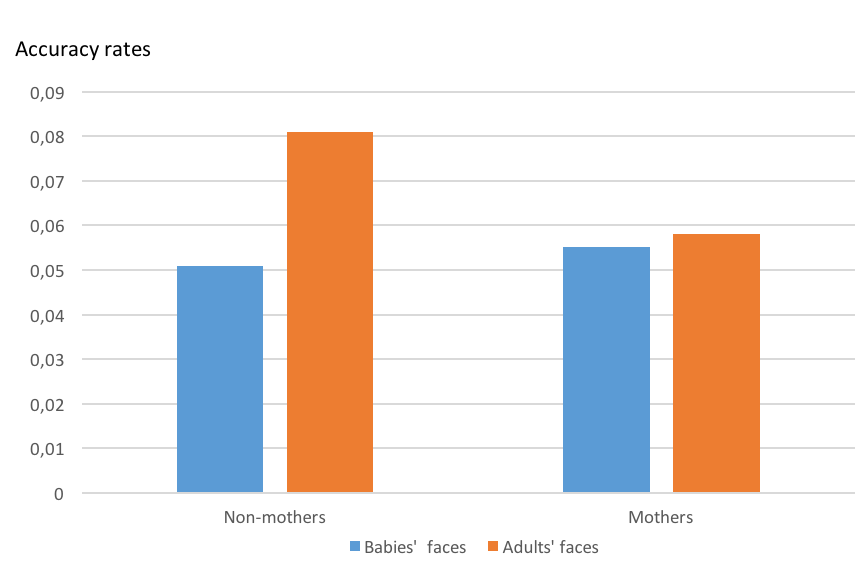
\includegraphics[width=\linewidth]{pictures/ACC_identity_motherhood.png}
%     \centering
%     \caption{Stroop effect of accuracy rates}
%   \end{subfigure}
%   \caption{The Stroop effects between different conditions of the sources of the facial expressions and status of the motherhood}
%   \label{fig.results.h3}
% \end{figure}

% \section{Additional effects}\label{sec.results.additional}
% As no significant difference in Stroop effect is found between when babies' faces are displayed and when adults' faces are displayed in the group of mothers, we intend to investigate whether the emotions of the facial expressions of the interference also has an influence over the effect. Therefore, we conduct two paired-samples t-tests. Significant results are found in the accuracy rates. 

\begin{figure}[!t]
  \centering
  \begin{subfigure}[b]{0.9\linewidth}
    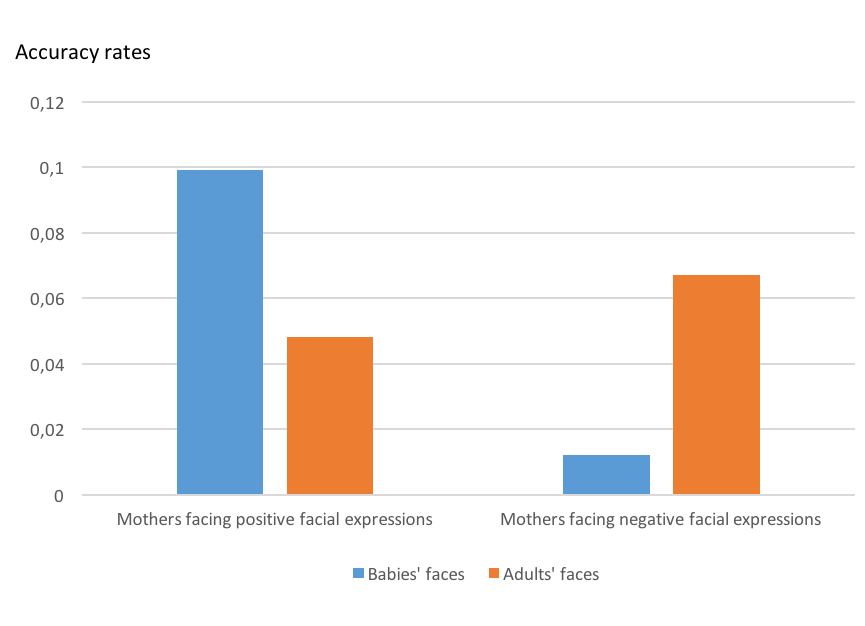
\includegraphics[width=\linewidth]{pictures/ACC_facialexp_identity.png}
    \caption{in the group of mothers}
  \end{subfigure}
  \begin{subfigure}[b]{0.9\linewidth}
    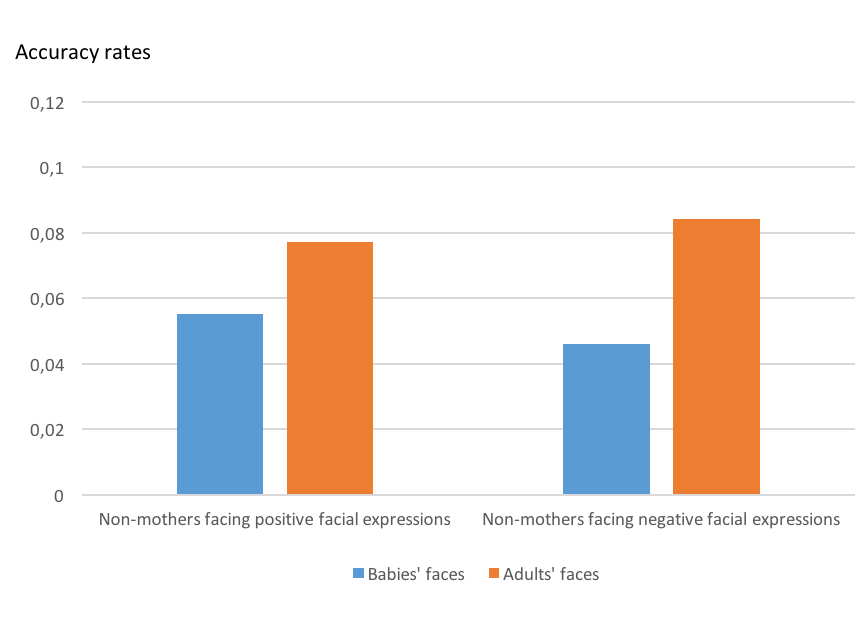
\includegraphics[width=\linewidth]{pictures/ACC_Nonmother_identity_facialexp.png}
    \caption{in the group of non-mothers}
  \end{subfigure}
  \caption{Stroop effect of the accuracy rates in the group of mothers as well as in the group of non-mothers when different sources and emotions of the facial expressions of the interference are presented}
  \label{fig.results.add}
\end{figure}







\chapter{Discussion}\label{chp.discussion}

As indicated in Section~\ref{chp.Criticism.Readers}, many readers see the rise of other-direction type at the expense of inner-direction type and therefore, lose the hopes and be pessimistic to the society. Thereafter, it is also important to reiterate that other-direction is not necessarily a bad thing, mainly discussed in~\ref{chp.reinterpretation}. What really matters is that we should be aware of its pull, so that being able to transcend and rise above it instead of letting it dominate our lives. Only by understanding something, one could free himself from it. Therefore, from this position of freedom and autonomy, the autonomous type of person is introduced, who is able to choose when to conform and when to resist.\\

As indicated in~\ref{chp.solution}, it is worth striving for the autonomous type, benefiting not only ourselves but also influencing the society and the next transition in the future. However, there are many challenges to become a autonomous person in this other-directed age. In this chapter two challenges are mainly introduced, namely the impact of the anxiety of the other-directed people and the impact of the mass media.\\

\textbf{Impact of the anxiety}
As indicated in Section~\ref{chp.reinterpretation.cost}, while striving for autonomous, we are suffering from a new form of anxiety about what to do and whom to trust. On one hand, the anxiety comes from the uncertain choice due to the large amounts of consuming possibilities. As is suggested by~\citeauthor{bude2014gesellschaft}, this anxiety, stem from the fear, could be defined as the feeling of helpless when we face the uncertainly, which is not derived so much from a ``powerful other'' but rather from the seemingly endless range of possibilities we face~\citep{bude2014gesellschaft}. One the other hand, as indicated in Section~\ref{chp.reinterpretation.cost}, other-directed people tend to compare their own experiences with different experiences that others are having, resulting in the uncertainty about whether the choice they made are properly. In order to reduce the impact of such anxiety, it is important to have confidence in ourselves, especially in making the choices, namely, instead of spending time comparing with others, we should also take the time listening to the inner voice and making our own choice, which follows the heart. Moreover, we should also be brave enough to do what we thought is appropriate, even it is different from what others normally do, since the society needs pioneers instead of followers.


%``Anxiety springs from the knowledge that everything is open but nothing is meaningless,'' he wrote, ``Our entire lives seem to be on the line at every single moment. The fear of simply drifting through life is hard to bear''. Every single ``wrong'' choice, such as choosing the ``wrong'' school, a ``wrong'' person to marry, could lead to the ``failure'' of life. We are struggling from the threat of the negative results instead of striving for success~\citep{bude2014gesellschaft}.

\textbf{Impact of The Mass Media}
Newspapers, books, magazines, comics, television, radio, movies, records, video games and the Internet, MP3 players, and smart phones, are all examples of what sociologists refer to as mass media--forms of a communication that reach a large audience. 

It is well-known that the media has literally become part of our everyday environment and is much more powerful and widespread than we thought, since the reach of the mass media has become so extensive, diverse and constant that it is difficult to find any person or any place in the world that does not have some regular exposure to media on daily basis~\citep{callero2017myth} and the society is more and more dominated by commerce and news. (refers to the Figure~\ref{discussion.fig.media})

\begin{figure}{t!}
  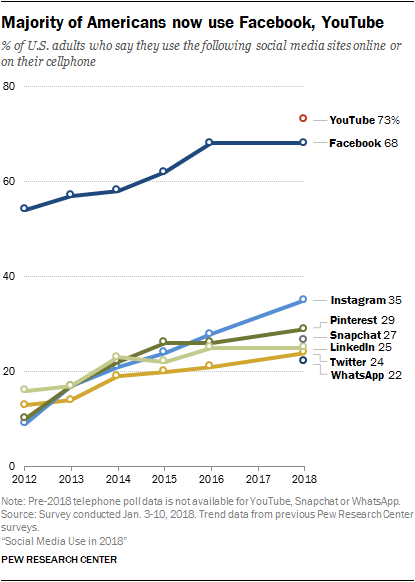
\includegraphics[width=\linewidth]{mass_media.png}
  \caption{The increase of the usage of the different kinds of social networks in the USA}
  \label{discussion.fig.media}
\end{figure}

Many worried about its threat to the individualism, since the other-directed people could easily be influenced by the mass media. Also written by David Riesman in the preface of the book ``The Lonely Crowd'', the gravest concern of the authors about the mass media, however, is not their long-run impact on culture, but the fact that the press, the news, the magazines, and particularly the newsreels have become far more ethnocentric and less parochial, which somewhat cover more foreign news, and only to smother it in the self-serving slogans and misleading the crowd. Edward W. Said also suggested that, ``despite the variety and the differences, and however much we proclaim the contrary, what the media produce is neither spontaneous nor completely ``free'': ``news'' does not just happen, pictures and ideas do not merely spring from reality into our eyes and minds, truth is not directly available, we do not have unrestrained variety at our disposal.'' In this information-saturated world, where the information could be both helpful and misleading, we need all the information we can get about all the information we are receiving and need to learn to pick the information we need and worth trusting, meanwhile, to be aware of the faking possibilities and think critical. 
% For example, as the online shopping is very popular and convenient, the ratings and reviews for a good are more and more important for the customers, which is also known by the sellers. Thereafter, they hire someone to rate the product high and write recommendations and compliments for the product, though it works not the same as is described. One one hand, the rating and reviewing system could help us to decide which to buy, on the other hand, some fake and misleading information may lead to the waste of money and time. 






 


			





\pagebreak

\appendix
%\addchaptertocentry{\appendixname}
\chapter{Information sheet and consent form}\label{appendix.consentinfo}
%\includegraphics[page=1-4,scale=0.8,trim=20 20 20 20,clip]{Appendix/consentform.pdf}
%\includegraphics[page=1,trim={70 0 0 },clip]{"Appendix/consentform"}
\begin{center}
\adjincludegraphics[page=1,trim={70 {.44\totalheight} 0 70},scale=0.9,clip]{"Appendix/consent_form_and_info_sheet"}
\newpage
\adjincludegraphics[page=1,trim={70 50 0 {.56\totalheight}},scale=0.9,clip]{"Appendix/consent_form_and_info_sheet"}
\newpage
\includegraphics[page=2,scale=0.9,trim={70 0 0 110},clip]{"Appendix/consent_form_and_info_sheet"}
\newpage
\includegraphics[page=3,scale=0.9,trim={70 0 0 110},clip]{"Appendix/consent_form_and_info_sheet"}
\newpage
\includegraphics[page=4,scale=0.9,trim={70 0 0 110},clip]{"Appendix/consent_form_and_info_sheet"}
\end{center}



\chapter{Demographic and handedness questionnaire}\label{appendix.demo}
\begin{center}
\adjincludegraphics[page=1,trim={70 {.44\totalheight} 0 70},scale=0.85,clip]{"Appendix/demographic_questionnaire"}
\newpage
\adjincludegraphics[page=1,trim={70 50 0 {.56\totalheight}},scale=0.85,clip]{"Appendix/demographic_questionnaire"}
% \includegraphics[page=1,scale=0.9,trim={70 0 0 70},clip]{"Appendix/demographic_questionnaire"}
\newpage
\includegraphics[page=2,scale=0.85,trim={30 0 0 70},clip]{"Appendix/demographic_questionnaire"}
\end{center}





\chapter{Between questionnaire for non-mothers}\label{appendix.between.nonmother}
\begin{center}
\includegraphics[page=1,scale=0.8,trim={60 90 0 90},clip]{"Appendix/Between_Task_Questions_Non-Mothers"}
\end{center}


\chapter{Between questionnaire for mothers}\label{appendix.between.mother}
\begin{center}
\includegraphics[page=1,scale=0.8,trim={60 90 0 90},clip]{"Appendix/Between_Task_Questions_Mothers"}
\end{center}





% \appendix 
% \addchaptertocentry{\appendixname}
% \chapter{}\label{appendix.consentinfo}
% \includegraphics[page=1-4,scale=0.8,trim=20 20 20 20,clip]{Appendix/consent_form_and_info_sheet.pdf}
% % 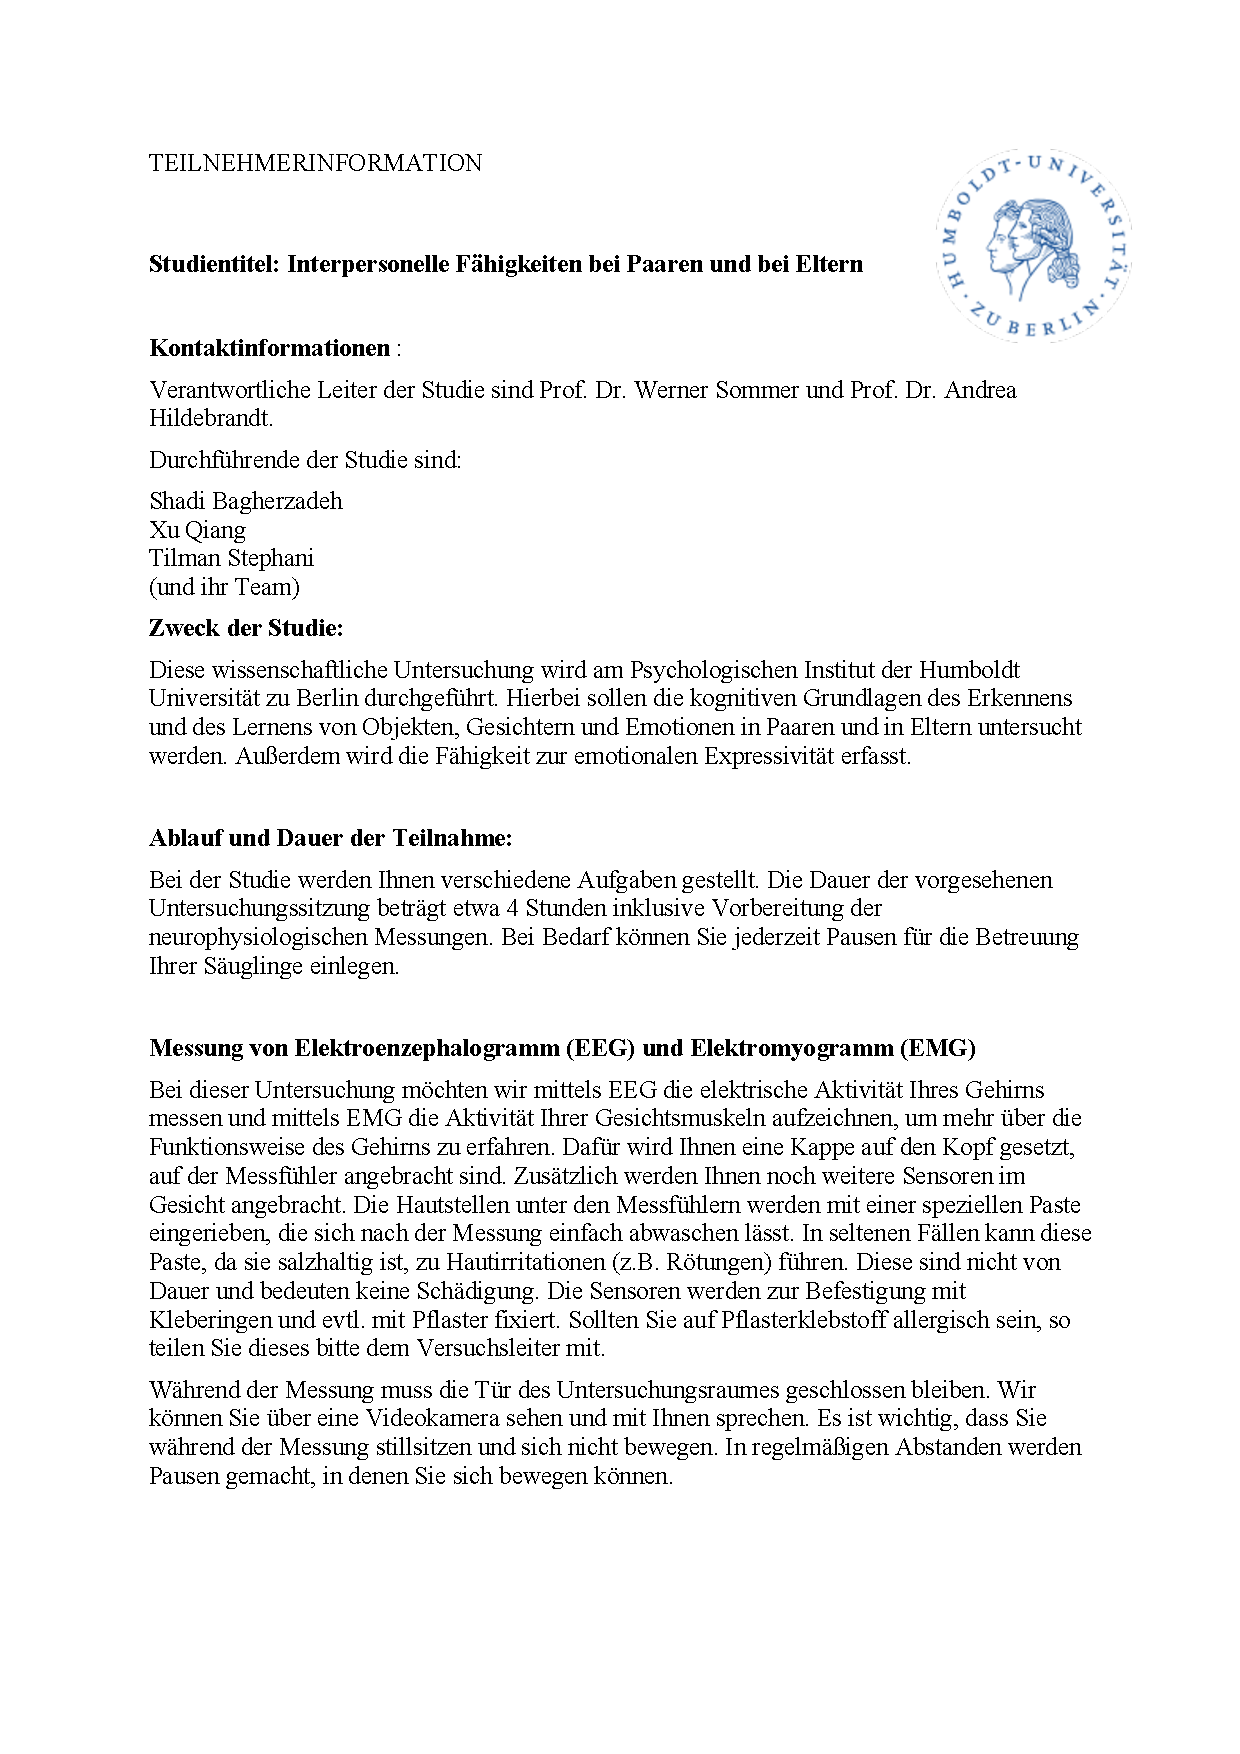
\includepdf[pages=1-4]{Appendix/consent_form_and_info_sheet.pdf}


% \chapter{}\label{appendix.demo}
% 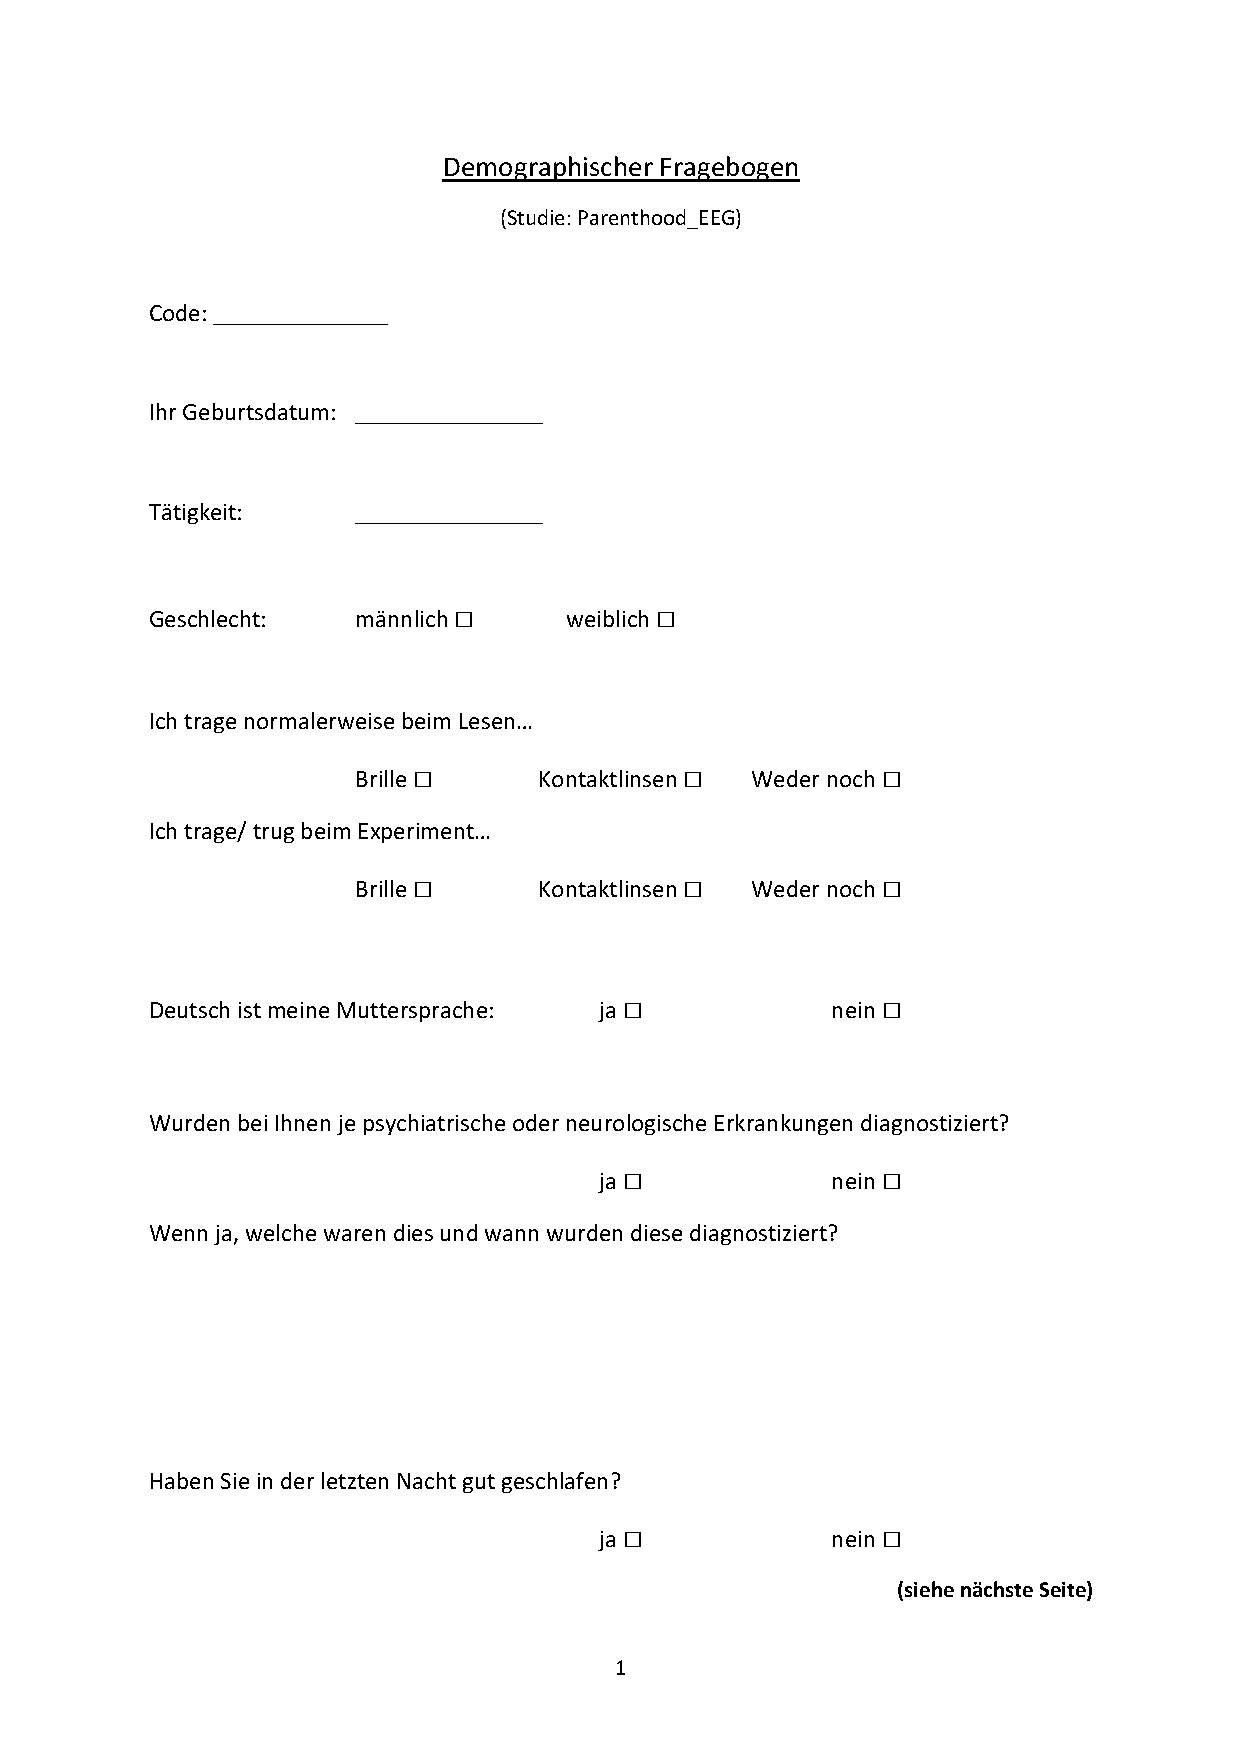
\includepdf[pages=1-2]{Appendix/demographic_questionnaire.pdf}
% \chapter{}\label{appendix.between.mother}
% 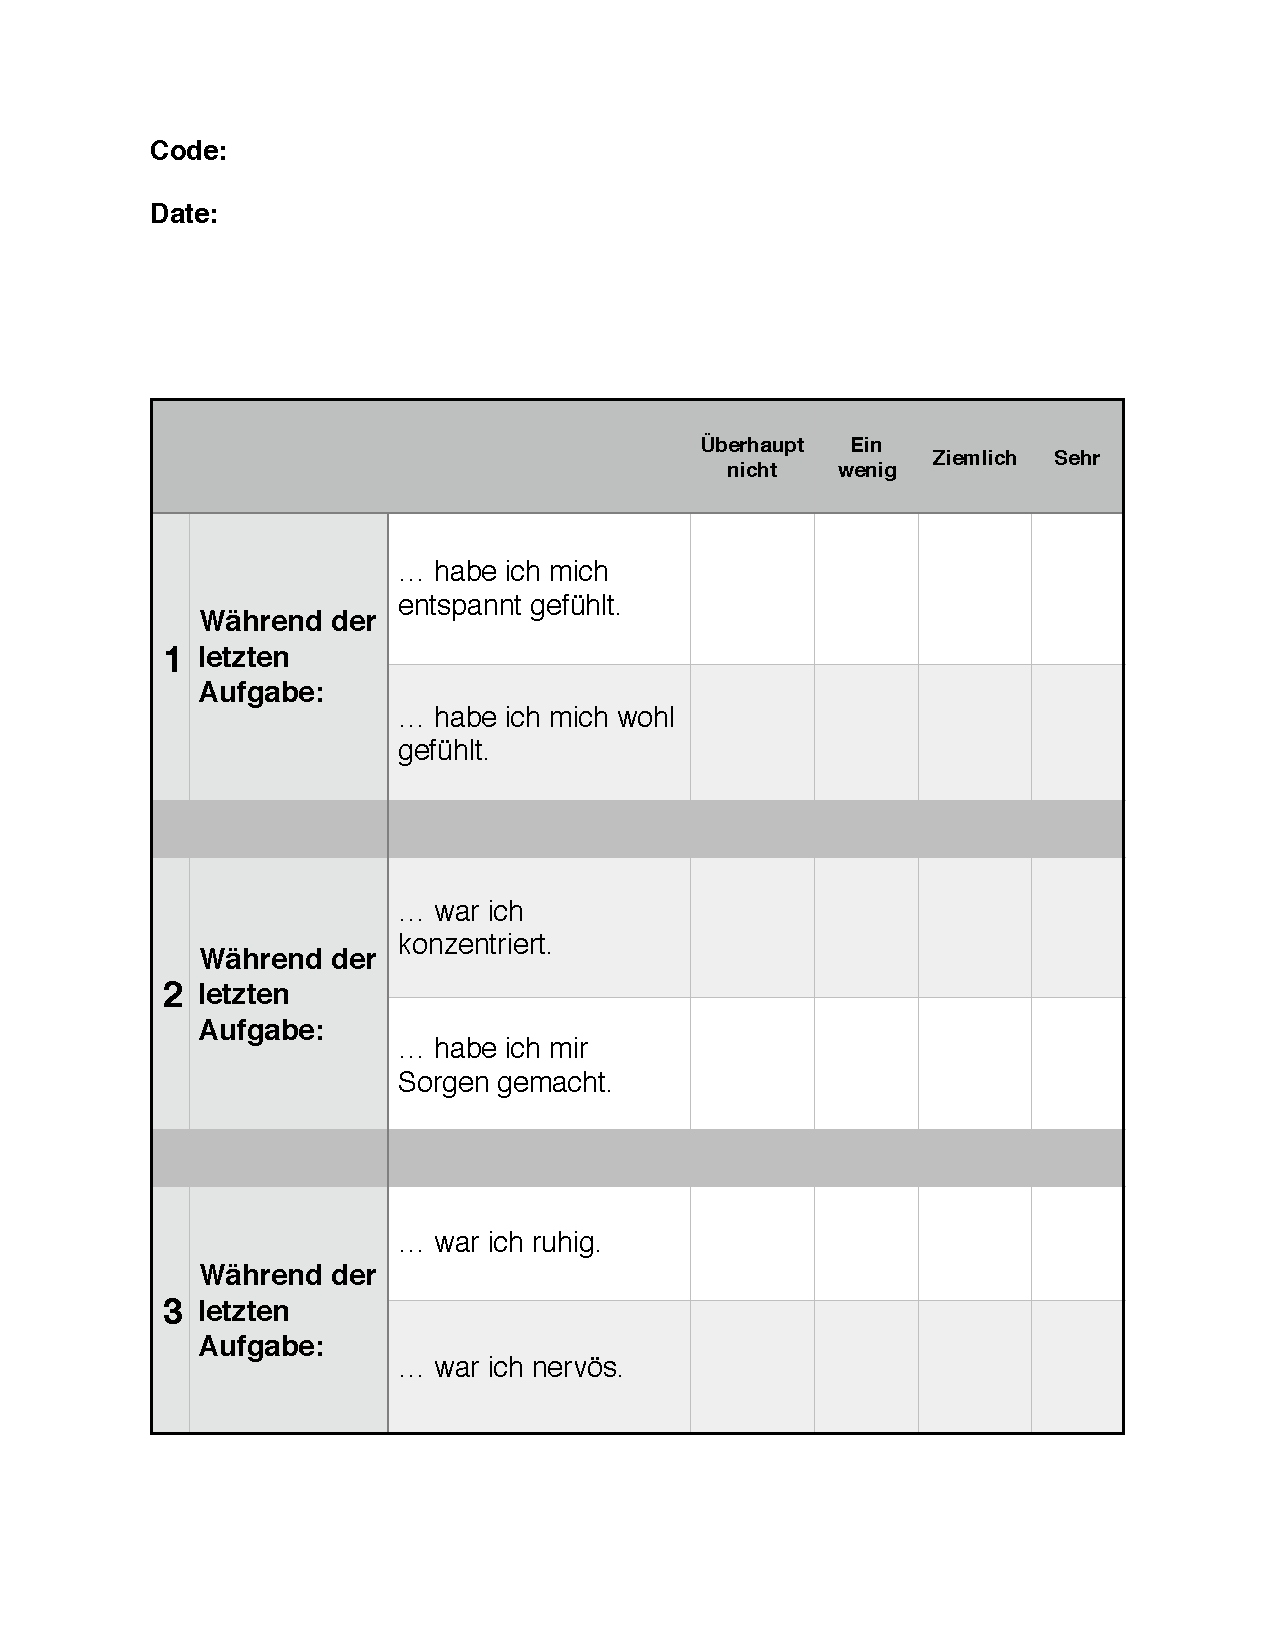
\includepdf[pages=1]{Appendix/Between_Task_Questions_Non-Mothers.pdf}
% \chapter{}\label{appendix.between.nonmother}
% 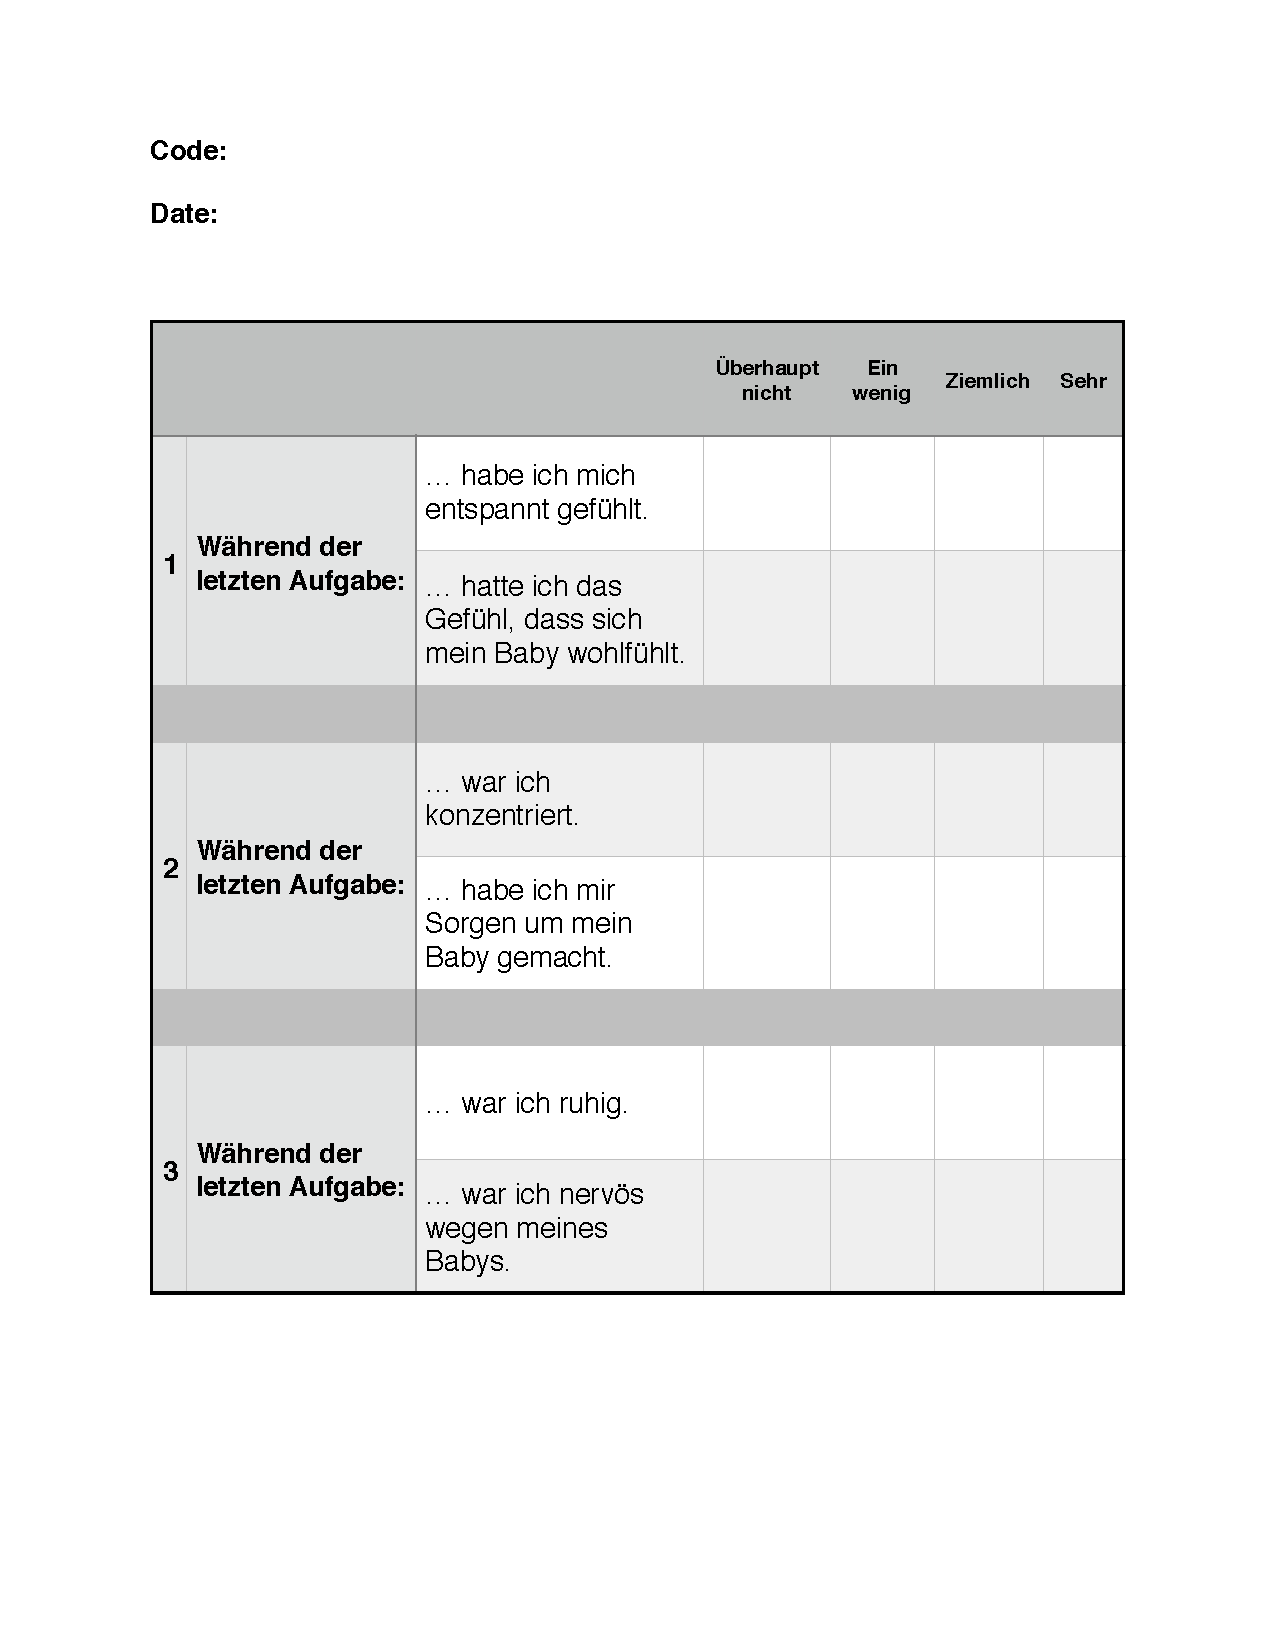
\includepdf[pages=1]{Appendix/Between_Task_Questions_Mothers.pdf}


\emergencystretch 1.5em
%\printbibliography[heading=bibintoc]
\bibliographystyle{apacite}
\bibliography{amycao.bib}




%\begin{declaration}
%\thispagestyle{empty}
%\addchaptertocentry{\authorshipname} 

%Ich versichere hiermit an Eides Statt, dass ich die von mir eingereichte Bachelor‐Arbeit bzw. die von mir namentlich gekennzeichneten Teile selbständig verfasst und ausschließlich die angegebenen Hilfsmittel benutzt habe.
% \\
% \\
% \\
% \noindent Signed:\\
% \rule[0.5em]{25em}{0.5pt} % This prints a line for the signature
 
% \noindent Date: Saarbrücken, den 16.04.2018\\
% \rule[0.5em]{25em}{0.5pt} % This prints a line to write the date
% \end{declaration}

\end{document}  
%----------------------------------------------------------------------------------------

